\chapter{Elementare Funktionen}

\setcounter{section}{10}
\setcounter{subsection}{0}
\setcounter{subsubsection}{1}
\setcounter{secnumdepth}{4}
\subsection{Sinus und Kosinus}
\href{https://youtu.be/8ApuQ6_PooA}{Video 01}\\
Es gibt eine eindeutige Funktion $ f:\mathbb{R}\longmapsto \mathbb{R} $ mit $ f+f''=0 $ und $ f(0)=0 $ sowie $ f'(0) =1$.\\
Wir schreiben $ f=\sin $ und $ f'=\cos $ und sagen Sinus bzw. Kosinus.\\
\begin{center}
	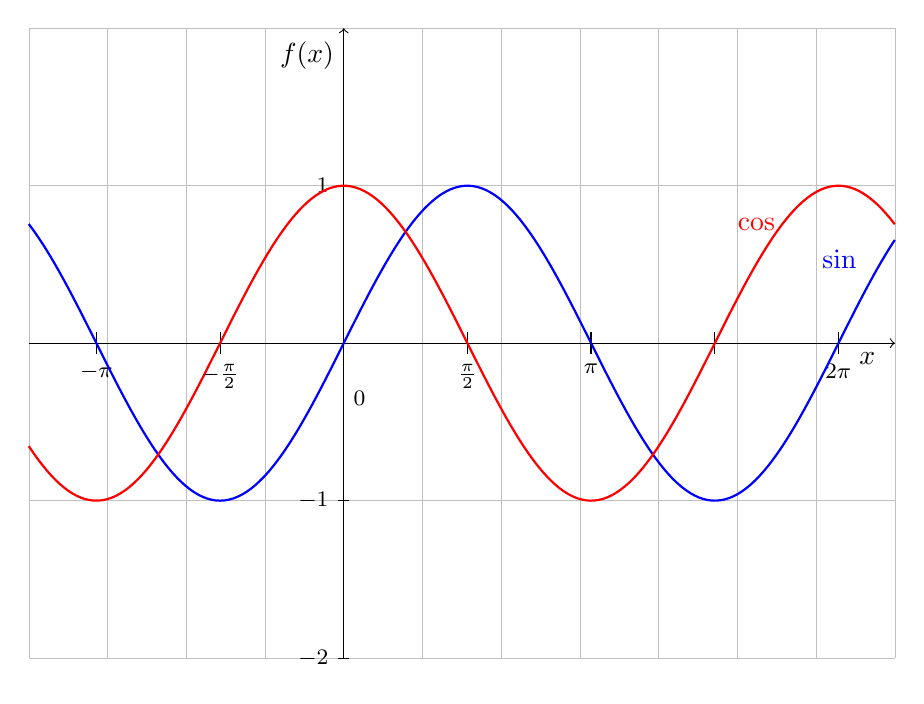
\begin{tikzpicture}[xscale=1,yscale=2][xscale=1,yscale=2]
	
	% Gitternetzlinien
	\draw[xstep=1cm, ystep=1cm, very thin, color=lightgray] (-4,2) grid (7,-2);
	% x-Achse
	\draw[->] (-4,0) -- (7,0) node[below,xshift=-1em] {$x$}; 
	%Zahlen auf x-Achse
	\foreach \x in {-3.14,-3.14/2}
	\draw[shift={(\x,0)},color=black] (0pt,2pt) -- (0pt,-2pt);
	\foreach \x in {3.14/2,3.14,4.71,6.28}
	\draw[shift={(\x,0)},color=black] (0pt,2pt) -- (0pt,-2pt);
	% y-Achse 
	\draw[->] (0,-2) -- (0,2) node[left,yshift=-1em] {$f(x)$};%node[above left]
	%Zahlen auf y-Achse
	\foreach \y in {-2,...,-1}
	\draw[shift={(0,\y)},color=black] (2pt,0pt) -- (-2pt,0pt) node[left] {\footnotesize $\y$};
	\foreach \y in {1,...,1}
	\draw[shift={(0,\y)},color=black] (2pt,0pt) -- (-2pt,0pt) node[left] {\footnotesize $\y$};
	%Ursprung
	\draw[color=black] (0pt,-10pt) node[right] {\footnotesize $0$};
	\draw[color=black] (3.14,-2pt) node[below] {\footnotesize $\pi$};
	\draw[color=black] (6.28,-2pt) node[below] {\footnotesize $2\pi$};
	\draw[color=black] (1.57,-2pt) node[below] {\footnotesize $\frac{\pi}{2}$};
	\draw[color=black] (-1.57,-2pt) node[below] {\footnotesize $-\frac{\pi}{2}$};
	\draw[color=black] (-3.14,-2pt) node[below] {\footnotesize $-\pi$};
	\draw[thick,color=blue] plot[samples=200, domain=-4:7] 
	(\x,{sin(\x r)}) node[below, xshift=-2em]{$\sin$};
	
	\draw[thick,color=red] plot[samples=200, domain=-4:7] 
	(\x,{cos(\x r)}) node[ xshift=-5em]{$\cos$};
	
	\end{tikzpicture}\\	
\end{center}
\underline{Eigenschaften}:\\
Für alle $ x\in \mathbb{R} $ gilt:\\
\begin{quote}
	\textbullet\;\;$ \sin(-x)=-\sin(x) $
	\begin{quote}
		ungerade Funktion \\
		punktsymmetrisch zum Koordinatenursprung\\
	\end{quote}
	\textbullet\;\;$ \cos(-x)=\cos(x) $
	\begin{quote}
		gerade Funktion\\
		symmetrisch zur y-Achse\\
	\end{quote}
	\newpage
	\noindent
	\textbullet\;\;$ \sin, \cos: \mathbb{R}\longmapsto[-1,1] $
	\begin{quote}
		$|\cos(x)|\leq 1$\\
		$|\sin(x)|\leq 1$\\
	\end{quote}
	\textbullet\;\;$\sin(k\cdot\pi)=0$ für $ k\in \mathbb{Z} $\\ \\
	\textbullet\;\;$\sin(\frac{\pi}{2}+k\frac{\pi}{2})=(-1)^k$ für $ k\in \mathbb{Z} $\\ \\
	\textbullet\;\;$\cos(\frac{\pi}{2}+k\frac{\pi}{2})=0 $ für $ k\in \mathbb{Z} $\\ \\
	\textbullet\;\;$ \cos(k\cdot\pi)=(-1)^k $ für $ k\in \mathbb{Z} $\\
\end{quote}
\subsubsection{Additionstheoreme des Sinus und Kosinus}\label{sec:Bezeichnung}
\href{https://youtu.be/Q-yJWE6P4uU}{Video 02}\\
Für $ x_1, x_2 \in\mathbb{R} $ gilt:\\ \\
(i)\;\;$ \sin(x_1+x_2)=\sin(x_1)\cdot \cos (x_2)+\sin(x_2)\cdot \cos(x_1)$\\ \\
(ii)\;$ \cos(x_1+x_2)=\cos(x_1)\cdot \cos(x_2) - \sin(x_1)\cdot \
sin(x_2)$\\ \\
Für $ x\in\mathbb{R} $ gilt:\\
\textbullet \;\;$\sin(x+\frac{\pi}{2})=\cos(x)$\\
\begin{align*}
\sin(x+\genfrac{}{}{}{2}{\pi }{2 })&\overset{(\mathrm{i})}{=}\sin(x)\cdot \underbrace {\cos(\genfrac{}{}{}{2}{\pi }{2 })}_{=0}+\underbrace {\sin(\genfrac{}{}{}{2}{\pi}{2 })}_{1}\cdot \cos(x)\\
&=\cos(x)
\end{align*}
\textbullet\;\;$\cos(2x)=\cos^2(x)-\sin^2(x)$\\
\begin{align*}
\cos(2x)=\cos(x+x)&\overset {(\mathrm{ii})}{=}\cos(x)\cdot\cos(x)-\sin(x)\cdot\sin(x)\\
&=\cos^2(x)-\sin^2(x)\\
\end{align*}
\textbullet \;\;$ \sin(2x)=2\sin(x)\cdot\cos(x) $\\
\begin{align*}
\sin(2x)=\sin(x+x)&\overset{(\mathrm{i})}{=}\sin(x)\cdot \cos(x)+\sin(x)\cdot \cos(x)\\
&=2\sin(x)\cdot\cos(x) \\
\end{align*}
\textbullet\;\;$\cos^2(x)+\sin^2(x)=1$\\
\newpage
\noindent
\subsubsection{ Aufgabe 1 zu den Additionstheoremen des Sinus und Kosinus}
\href{https://youtu.be/fVSPz-IaCqA}{Video 03}\\
Zeige für alle $ x\in\mathbb{R} $ gilt $ \cos^2(x)+\sin^2(x) =1$.\\ \\
Es gilt für alle $ x\in\mathbb{R} $:\\
\begin{align*}
\mathrm{e}^{\mathrm{i}x}=\cos(x)+\mathrm{i}\cdot\sin(x)
\end{align*}
Betrachte:\\
\begin{align*}
\cos^2(x)+\sin^2(x)&= \cos^2(x)\underbrace {-\mathrm{i^2}}_{=1}\cdot \sin^2(x)\;\;|\text{\tiny $\mathrm{i}^2=-1\Rightarrow -\mathrm{i}^2=1$ }\\
&=\cos^2(x)-(\mathrm{i}\cdot \sin(x))^2\;\;|\text{\tiny mit 3. binomischer Formel }\\
&=\bigg(\cos(x)-\mathrm{i}\cdot \sin(x\big)\bigg)\bigg(\cos(x)+\mathrm{i}\cdot \sin(x)\bigg)\;\;|\text{\tiny $ \cos(x)=\cos(-x),-\mathrm{i}\cdot \sin(x)=+\mathrm{i}\cdot\sin(-x) $ }\\
&=\bigg(\cos(-x)+\mathrm{i}\cdot\sin(-x)\bigg)\bigg(\cos(x)+\mathrm{i}\cdot \sin(x)\bigg)\;\;|\text{\tiny $\mathrm{e}^{\mathrm{i}x}=\cos(x)+\mathrm{i}\cdot\sin(x)  $}\\
&=\mathrm{e}^{-\mathrm{i}x}\cdot\mathrm{e}^{\mathrm{i}x}=\mathrm{e}^0=1_{_{\Square}}
\end{align*}
\subsubsection{ Aufgabe 2 zu den Additionstheoremen des Sinus und Kosinus}
\href{https://youtu.be/Ibl3wG8lgyE}{Video 04}\\
Bestimme alle $ x\in\mathbb{R} $ mit $ \sqrt{2}\sin(x)-\sin(2x)=0 $.\\
Bemerkung:\\
\begin{center}
	\renewcommand{\arraystretch}{1.8}
	\( \begin{array}{l|c|c|c|c|c} 
	x&0\overset{\wedge}{=}0^\circ&\frac{\pi}{6}\overset{\wedge}{=}30^\circ&\frac{\pi}{4}\overset{\wedge}{=}45^\circ&\frac{\pi}{3}\overset{\wedge}{=}60^\circ&\frac{\pi}{2}\overset{\wedge}{=}90^\circ\\
	\hline
	\sin(x)&\frac{\sqrt{0}}{2}&\frac{\sqrt{1}}{2}&\frac{\sqrt{2}}{2}&\frac{\sqrt{3}}{2}&\frac{\sqrt{4}}{2}\\
	\hline
	\cos(x)&\frac{\sqrt{4}}{2}&\frac{\sqrt{3}}{2}&\frac{\sqrt{2}}{2}&\frac{\sqrt{1}}{2}&\frac{\sqrt{0}}{2}
	\end{array} \)	
\end{center}
\begin{align*}
&\sqrt{2}\sin(x)-\sin(2x)=0\\
&\Leftrightarrow\\
&\sqrt{2}\sin(x)=\sin(2x)\;\;|\text{\tiny $ \sin(2x)=2\sin(x)\cos(x) $ }\\
&\sqrt{2}\sin(x)=2\sin(x)\cos(x)\\
\end{align*}
\underline{1.Fall:} $ \sin(x)\neq 0 $\\
\begin{align*}
\sqrt{2}\sin(x)&=2\sin(x)\cos(x)\;\;|\text{\tiny $\div \sin(x)  $  }\\
\sqrt{2}&=2\cos(x)\\
\frac{\sqrt{2}}{2}&=\cos(x)\\
\end{align*}
\begin{quote}
	D.h. eine Lösung bei $ x=\frac{\pi}{4}=\cos(\frac{\sqrt{2}}{2}) $ und alle Lösungen bei:\\
	\begin{align*}
	\text{Es gilt: }&\cos(x+k2\pi)=\cos(x)\;\;\text{mit }\;\; k\in\mathbb{Z}\\
	&\Rightarrow \cos(\genfrac{}{}{}{2}{\pi }{4 }+k2\pi) \;\;\text{mit }\;\;k\in\mathbb{Z}\\
	\end{align*}
\end{quote}
\underline{1.Fall:} $ \sin(x)= 0 $\\
\begin{align*}
\sqrt{2}\sin(x)=2\sin(x)\cos(x)=0\\
\end{align*}
\begin{quote}
	Immer erfüllt für alle Nullstellen von $ \sin(x) $ mit $ x=j\cdot\pi $ mit $ j\in  \mathbb{Z} $
\end{quote}
Die Lösungsmenge ist:\\
\begin{align*}
\mathbb{L}=\{\genfrac{}{}{}{2}{\pi }{4 }+k \cdot 2 \pi, j\cdot \pi | k,j\in  \mathbb{Z}\}
\end{align*}
oder:\
\begin{align*}
\mathbb{L}=\underset{k\in \mathbb{Z}}{\bigcup}\{\genfrac{}{}{}{2}{\pi}{4}+k2\pi,k\pi\}\\
\end{align*}
\subsection{Der Tangens und Kotangens}
\subsubsection{Der Tangens}
\href{https://youtu.be/zwQ_9S4sgro}{Video 05}\\
Defintion des Tangens:\\
\begin{align*}
\tan(x)=\frac{\sin(x)}{\cos(x)}\;\;\text{für }\;\;x\neq \frac{\pi}{2}+k\cdot\pi,\; k\in \mathbb{Z}
\end{align*}
Diese Funktion ist $ \pi- $periodisch.\\
Es gilt:\\
\begin{align*}
\tan(x+\pi)=\tan(x)
\end{align*}
\begin{center}
	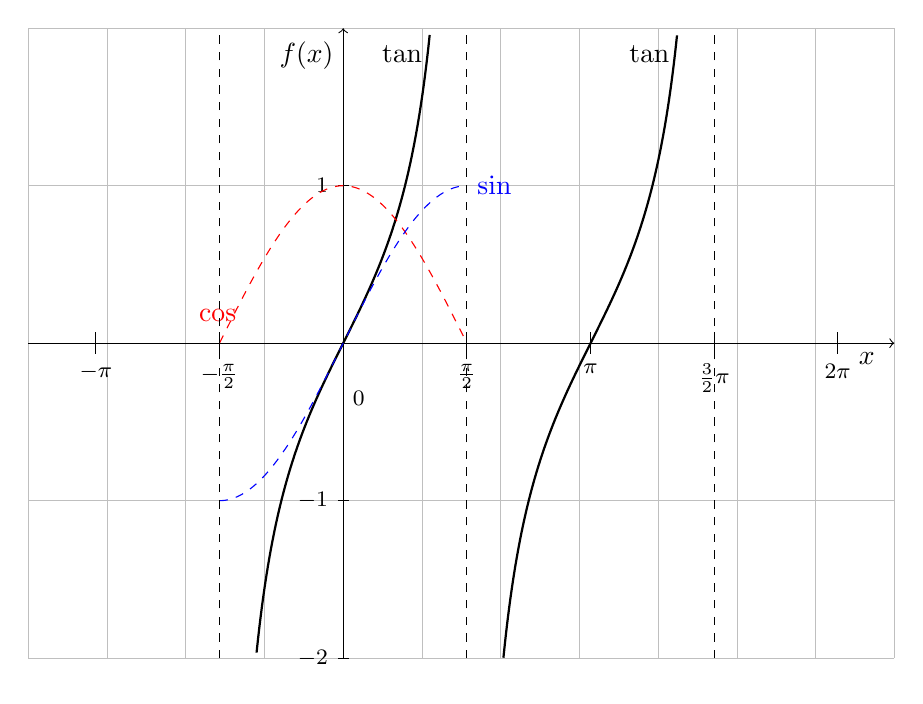
\begin{tikzpicture}[xscale=1,yscale=2]
	
	% Gitternetzlinien
	\draw[xstep=1cm, ystep=1cm, very thin, color=lightgray] (-4,2) grid (7,-2);
	% x-Achse
	\draw[->] (-4,0) -- (7,0) node[below,xshift=-1em] {$x$}; 
	%Zahlen auf x-Achse
	\foreach \x in {-3.14,-3.14/2}
	\draw[shift={(\x,0)},color=black] (0pt,2pt) -- (0pt,-2pt);
	\foreach \x in {3.14/2,3.14,4.71,6.28}
	\draw[shift={(\x,0)},color=black] (0pt,2pt) -- (0pt,-2pt);
	% y-Achse 
	\draw[->] (0,-2) -- (0,2) node[left,yshift=-1em] {$f(x)$};%node[above left]
	%Zahlen auf y-Achse
	\foreach \y in {-2,...,-1}
	\draw[shift={(0,\y)},color=black] (2pt,0pt) -- (-2pt,0pt) node[left] {\footnotesize $\y$};
	\foreach \y in {1,...,1}
	\draw[shift={(0,\y)},color=black] (2pt,0pt) -- (-2pt,0pt) node[left] {\footnotesize $\y$};
	%Ursprung
	\draw[color=black] (0pt,-10pt) node[right] {\footnotesize $0$};
	\draw[color=black] (3.14,-2pt) node[below] {\footnotesize $\pi$};
	\draw[color=black] (6.28,-2pt) node[below] {\footnotesize $2\pi$};
	\draw[color=black] (1.57,-2pt) node[below] {\footnotesize $\frac{\pi}{2}$};
	\draw[color=black] (-1.57,-2pt) node[below] {\footnotesize $-\frac{\pi}{2}$};
	\draw[color=black] (-3.14,-2pt) node[below] {\footnotesize $-\pi$};
	\draw[color=black] (3*3.14/2,-2pt) node[below] {\footnotesize $\frac{3}{2}\pi$};
	\draw[thick,color=black] plot[samples=200, domain=-2.2/2:2.2/2] 
	(\x,{tan(\x r)}) node[below, xshift=-1em]{$\tan$};
	\draw[thick,color=black] plot[samples=200, domain=4.07/2:4.24] 
	(\x,{tan(\x r)}) node[below, xshift=-1em]{$\tan$};
	\draw[dashed,color=red] plot[samples=200, domain=-3.14/2:3.14/2] 
	(\x,{cos(\x r)}) node[ xshift=-9em,yshift=1em]{$\cos$};
	\draw[dashed,color=blue] plot[samples=200, domain=-3.14/2:3.14/2] 
	(\x,{sin(\x r)}) node[ xshift=1em]{$\sin$};
	\draw[dashed,color=black] (-3.14/2,-2)--(-3.14/2,2);
	\draw[dashed,color=black] (3.14/2,-2)--(3.14/2,2);
	\draw[dashed,color=black] (3.14/2+3.14,-2)--(3.14/2+3.14,2);
	\end{tikzpicture}\\	
\end{center}
Für die Abbildung der Hauptperiode gilt:\\
\begin{align*}
\tan:\;]\genfrac{}{}{}{2}{-\pi }{2},\genfrac{}{}{}{2}{\pi}{2}[\;\;\text{mit }\;\; \longmapsto \mathbb{R}\;\;x\longmapsto \frac{\sin(x)}{\cos(x)}
\end{align*}
Der Tangens ist als Komposition diffbarer Funktionen diffbar.\\
\begin{align*}
\tan'(x)=\bigg(\frac{\sin(x)}{\cos(x)}\bigg)'&=\frac{\cos(x)\cos(x)-\sin(x)(-\sin(x))}{\cos^2(x)}\\
&=\frac{\cos^2(x)+\sin^2(x)}{\cos^2(x)}\;\;|\text{\tiny $ \cos^2(x)+\sin^2(x)=1 $ }\\
&=\frac{1}{\cos^2(x)}\\
&=\frac{\cos^2(x)}{\cos^2(x)}+\frac{\sin^2(x)}{\cos^2(x)}=1+\tan^2(x)>0\\
\end{align*}
Nach dem Monotoniekriterium ist der Tangens streng monoton steigend.\\
\subsubsection{Der Kotangens}
\href{https://youtu.be/3N8L_ze4y2o}{Video 06}\\
Definition des Kotangens:\\
\begin{align*}
\cot(x+k\pi)=\cot(x)\;\;\text{für }\;\; x\neq k\pi, k\in \mathbb{Z}
\end{align*}
\begin{center}
	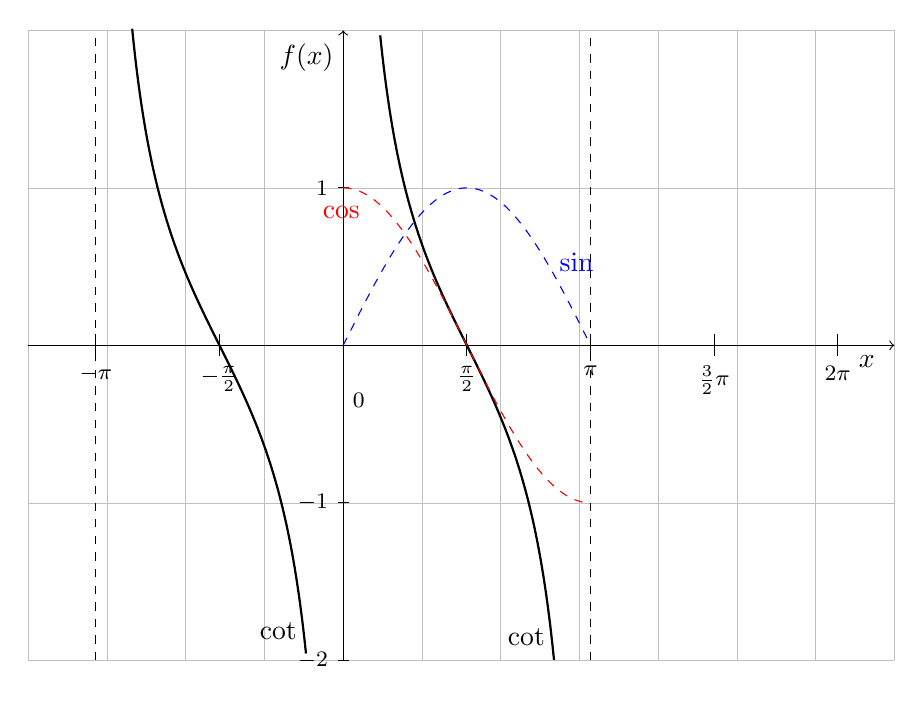
\begin{tikzpicture}[xscale=1,yscale=2]
	
	% Gitternetzlinien
	\draw[xstep=1cm, ystep=1cm, very thin, color=lightgray] (-4,2) grid (7,-2);
	% x-Achse
	\draw[->] (-4,0) -- (7,0) node[below,xshift=-1em] {$x$}; 
	%Zahlen auf x-Achse
	\foreach \x in {-3.14,-3.14/2}
	\draw[shift={(\x,0)},color=black] (0pt,2pt) -- (0pt,-2pt);
	\foreach \x in {3.14/2,3.14,4.71,6.28}
	\draw[shift={(\x,0)},color=black] (0pt,2pt) -- (0pt,-2pt);
	% y-Achse 
	\draw[->] (0,-2) -- (0,2) node[left,yshift=-1em] {$f(x)$};%node[above left]
	%Zahlen auf y-Achse
	\foreach \y in {-2,...,-1}
	\draw[shift={(0,\y)},color=black] (2pt,0pt) -- (-2pt,0pt) node[left] {\footnotesize $\y$};
	\foreach \y in {1,...,1}
	\draw[shift={(0,\y)},color=black] (2pt,0pt) -- (-2pt,0pt) node[left] {\footnotesize $\y$};
	%Ursprung
	\draw[color=black] (0pt,-10pt) node[right] {\footnotesize $0$};
	\draw[color=black] (3.14,-2pt) node[below] {\footnotesize $\pi$};
	\draw[color=black] (6.28,-2pt) node[below] {\footnotesize $2\pi$};
	\draw[color=black] (1.57,-2pt) node[below] {\footnotesize $\frac{\pi}{2}$};
	\draw[color=black] (-1.57,-2pt) node[below] {\footnotesize $-\frac{\pi}{2}$};
	\draw[color=black] (-3.14,-2pt) node[below] {\footnotesize $-\pi$};
	\draw[color=black] (3*3.14/2,-2pt) node[below] {\footnotesize $\frac{3}{2}\pi$};
	\draw[thick,color=black] plot[samples=200, domain=0.47:2.68] 
	(\x,{cot(\x r)}) node[below, xshift=-1em,yshift=15]{$\cot$};
	\draw[thick,color=black] plot[samples=200, domain=-2.68:-0.47] 
	(\x,{cot(\x r)}) node[below, xshift=-1em,yshift=15]{$\cot$};
	\draw[dashed,color=red] plot[samples=200, domain=0:3.14] 
	(\x,{cos(\x r)}) node[ xshift=-9em,yshift=10.5em]{$\cos$};
	\draw[dashed,color=blue] plot[samples=200, domain=0:3.14] 
	(\x,{sin(\x r)}) node[ xshift=-0.5em,yshift=3em]{$\sin$};
	\draw[dashed,color=black] (-3.14,-2)--(-3.14,2);
	\draw[dashed,color=black] (3.14,-2)--(3.14,2);
	%\draw[dashed,color=black] (3.14/2+3.14,-2)--(3.14/2+3.14,2);
	\end{tikzpicture}\\	
\end{center}
Für die Abbildung der Hauptperiode gilt:\\
\begin{align*}
\cot:\;]0,\pi[ \;\longmapsto \mathbb{R}\;\;\text{für }\;\;x\longmapsto\frac{\cos(x)}{\sin(x)}
\end{align*}
Der Kotangens ist als Komposition diffbarer Funktionen diffbar.\\
\begin{align*}
\cot'(x)=\bigg(\frac{\cos(x)}{\sin(x)}\bigg)'&=\frac{-\sin^2(x)-\cos^2(x)}{\sin^2(x)}\\
&=\frac{-(\sin^2(x)+\cos^2(x))}{\sin^2(x)}=-\frac{1}{\sin^2(x)}\\
&=-1-\cot^2(x)<0\\
\end{align*}
Nach dem Monotoniekriterium ist der Kotangens streng monoton fallend.\\
\subsubsection{Arcussinus und Arcuskosinus}
\href{https://youtu.be/WWMBFDeShK4}{Video 07}\\
$\blacktriangleright$ Umkehrfunktion vom Kosinus.\\
\begin{quote}
	
	\begin{center}
		
		
		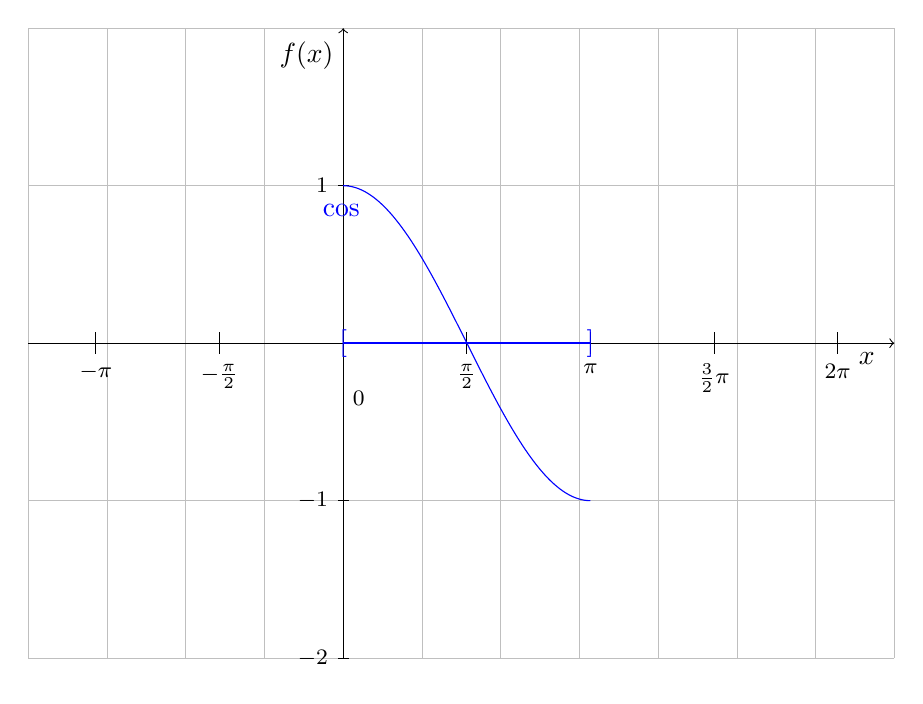
\begin{tikzpicture}[xscale=1,yscale=2]
		
		% Gitternetzlinien
		\draw[xstep=1cm, ystep=1cm, very thin, color=lightgray] (-4,2) grid (7,-2);
		% x-Achse
		\draw[->] (-4,0) -- (7,0) node[below,xshift=-1em] {$x$}; 
		%Zahlen auf x-Achse
		\foreach \x in {-3.14,-3.14/2}
		\draw[shift={(\x,0)},color=black] (0pt,2pt) -- (0pt,-2pt);
		\foreach \x in {3.14/2,3.14,4.71,6.28}
		\draw[shift={(\x,0)},color=black] (0pt,2pt) -- (0pt,-2pt);
		% y-Achse 
		\draw[->] (0,-2) -- (0,2) node[left,yshift=-1em] {$f(x)$};%node[above left]
		%Zahlen auf y-Achse
		\foreach \y in {-2,...,-1}
		\draw[shift={(0,\y)},color=black] (2pt,0pt) -- (-2pt,0pt) node[left] {\footnotesize $\y$};
		\foreach \y in {1,...,1}
		\draw[shift={(0,\y)},color=black] (2pt,0pt) -- (-2pt,0pt) node[left] {\footnotesize $\y$};
		%Ursprung
		\draw[color=black] (0pt,-10pt) node[right] {\footnotesize $0$};
		\draw[color=black] (3.14,-2pt) node[below] {\footnotesize $\pi$};
		\draw[color=black] (6.28,-2pt) node[below] {\footnotesize $2\pi$};
		\draw[color=black] (1.57,-2pt) node[below] {\footnotesize $\frac{\pi}{2}$};
		\draw[color=black] (-1.57,-2pt) node[below] {\footnotesize $-\frac{\pi}{2}$};
		\draw[color=black] (-3.14,-2pt) node[below] {\footnotesize $-\pi$};
		\draw[color=black] (3*3.14/2,-2pt) node[below] {\footnotesize $\frac{3}{2}\pi$};
		
		\draw[color=blue] plot[samples=200, domain=0:3.14] 
		(\x,{cos(\x r)}) node[ xshift=-9em,yshift=10.5em]{$\cos$};
		\draw[color=blue,thick] (0pt,0pt) node {$[$};
		\draw[color=blue,thick] (3.14,0pt) node { $]$};
		\draw[color=blue,thick] (0,0pt)--(3.14,0);
		%\draw[dashed,color=black] (-3.14,-2)--(-3.14,2);
		%\draw[dashed,color=black] (3.14,-2)--(3.14,2);
		%\draw[dashed,color=black] (3.14/2+3.14,-2)--(3.14/2+3.14,2);
		\end{tikzpicture}\\	
		Umkehrbahr nur in diesen Intervall, wegen der Bijektivität \\
		$\cos:[0,\pi]\longmapsto[-1,1] $\\ 
	\end{center}
	\newpage
	\noindent
	\begin{align*}
	\arccos:=\cos^{-1}:[-1,1]\longmapsto[0,\pi]
	\end{align*}
	\begin{center}
		\begin{tikzpicture}[xscale=3, yscale=2]
		
		% Gitternetzlinien
		\draw[xstep=1cm, ystep=1cm, very thin, color=lightgray] (-2,4) grid (2,-1);
		% x-Achse
		\draw[->] (-2,0) -- (2,0) node[below,xshift=-1em] {$x$}; 
		%Zahlen auf x-Achse
		\foreach \x in {-1,...,-1}
		\draw[shift={(\x,0)},color=black] (0pt,2pt) -- (0pt,-2pt) node[below] {\footnotesize $\x$};
		\foreach \x in {1,...,1}
		\draw[shift={(\x,0)},color=black] (0pt,2pt) -- (0pt,-2pt) node[below] {\footnotesize $\x$};
		% y-Achse 
		\draw[->] (0,-1) -- (0,4) node[left,yshift=-1em] {$f(x)$};%node[above left]
		%Zahlen auf y-Achse
		\foreach \y in {-1,...,-1}
		\draw[shift={(0,\y)},color=black] (2pt,0pt) -- (-2pt,0pt) node[left] {\footnotesize $\y$};
		\foreach \y in {1,...,3}
		\draw[shift={(0,\y)},color=black] (2pt,0pt) -- (-2pt,0pt) node[left] {\footnotesize $\y$};
		%Ursprung
		\draw[color=black] (0pt,-10pt) node[right] {\footnotesize $0$};
		
		\draw[thick,color=blue] plot[samples=200, domain=-0.999:0.999] 
		(\x,{rad(acos(\x ))}) node[yshift=1, xshift=2em] {$\arccos$};
		
		\draw[color=black] (2pt,3.14) -- (-2pt,3.14) node[left] {\footnotesize $\pi$};
		
		\draw[color=black] (2pt,3.14/2) -- (-2pt,3.14/2) node[left] {\footnotesize $\frac{\pi}{2}$};
		
		\end{tikzpicture}\\
		\begin{align*}
		\arccos'(x)=\frac{-1}{\sqrt{1-x^2}}
		\end{align*}
		
	\end{center}
\end{quote}
$\blacktriangleright$ Umkehrfunktion vom Sinus.\\
\begin{quote}
	\begin{center}
		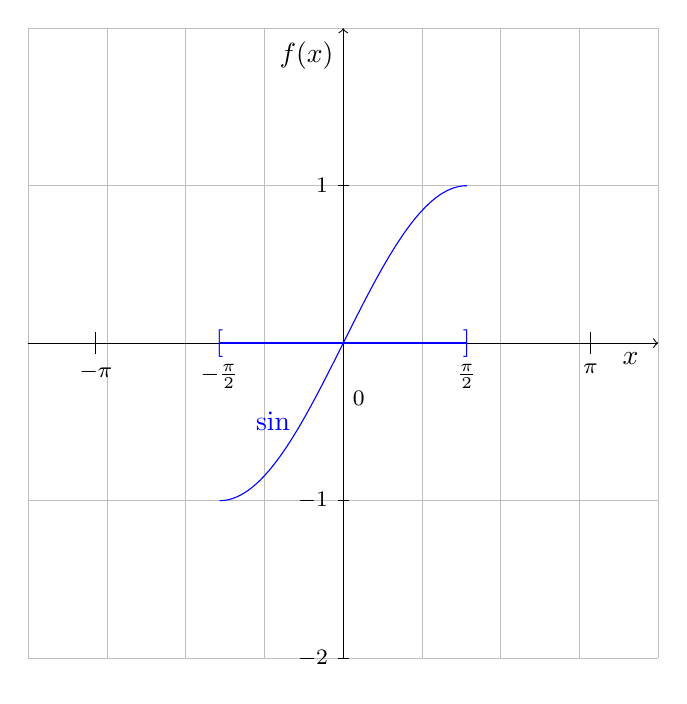
\begin{tikzpicture}[xscale=1,yscale=2]
		
		% Gitternetzlinien
		\draw[xstep=1cm, ystep=1cm, very thin, color=lightgray] (-4,2) grid (4,-2);
		% x-Achse
		\draw[->] (-4,0) -- (4,0) node[below,xshift=-1em] {$x$}; 
		%Zahlen auf x-Achse
		\foreach \x in {-3.14,3.14}
		\draw[shift={(\x,0)},color=black] (0pt,2pt) -- (0pt,-2pt);
		\foreach \x in {3.14/2,3.14}
		\draw[shift={(\x,0)},color=black] (0pt,2pt) -- (0pt,-2pt);
		% y-Achse 
		\draw[->] (0,-2) -- (0,2) node[left,yshift=-1em] {$f(x)$};%node[above left]
		%Zahlen auf y-Achse
		\foreach \y in {-2,...,-1}
		\draw[shift={(0,\y)},color=black] (2pt,0pt) -- (-2pt,0pt) node[left] {\footnotesize $\y$};
		\foreach \y in {1,...,1}
		\draw[shift={(0,\y)},color=black] (2pt,0pt) -- (-2pt,0pt) node[left] {\footnotesize $\y$};
		%Ursprung
		\draw[color=black] (0pt,-10pt) node[right] {\footnotesize $0$};
		\draw[color=black] (3.14,-2pt) node[below] {\footnotesize $\pi$};
		%\draw[color=black] (6.28,-2pt) node[below] {\footnotesize $2\pi$};
		\draw[color=black] (1.57,-2pt) node[below] {\footnotesize $\frac{\pi}{2}$};
		\draw[color=black] (-1.57,-2pt) node[below] {\footnotesize $-\frac{\pi}{2}$};
		\draw[color=black] (-3.14,-2pt) node[below] {\footnotesize $-\pi$};
		%\draw[color=black] (3*3.14/2,-2pt) node[below] {\footnotesize $\frac{3}{2}\pi$};
		
		\draw[color=blue] plot[samples=200, domain=-3.14/2:3.14/2] 
		(\x,{sin(\x r)}) node[ xshift=-7em,yshift=-8.5em]{$\sin$};
		\draw[color=blue,thick] (-3.14/2,0pt) node {$[$};
		\draw[color=blue,thick] (3.14/2,0pt) node { $]$};
		\draw[color=blue,thick] (-3.14/2,0)--(3.14/2,0);
		%\draw[dashed,color=black] (-3.14,-2)--(-3.14,2);
		%\draw[dashed,color=black] (3.14,-2)--(3.14,2);
		%\draw[dashed,color=black] (3.14/2+3.14,-2)--(3.14/2+3.14,2);
		\end{tikzpicture}\\	
		Umkehrbar nur in diesen Intervall, wegen der Bijektivität.\\
		$ \sin:[-\frac{\pi}{2},+\frac{\pi}{2}]\longmapsto[-1,1] $\\
	\end{center}
	\newpage
	\noindent
	\begin{align*}
	\arcsin:=\sin^{-1}:[-1,1]\longmapsto[-\genfrac{}{}{}{1.7}{\pi}{2 },\genfrac{}{}{}{1.7}{\pi }{2}]
	\end{align*}
	\begin{center}
		\begin{tikzpicture}[xscale=3, yscale=2]
		
		% Gitternetzlinien
		\draw[xstep=1cm, ystep=1cm, very thin, color=lightgray] (-2,2) grid (2,-2);
		% x-Achse
		\draw[->] (-2,0) -- (2,0) node[below,xshift=-1em] {$x$}; 
		%Zahlen auf x-Achse
		\foreach \x in {-1,...,-1}
		\draw[shift={(\x,0)},color=black] (0pt,2pt) -- (0pt,-2pt) node[below] {\footnotesize $\x$};
		\foreach \x in {1,...,1}
		\draw[shift={(\x,0)},color=black] (0pt,2pt) -- (0pt,-2pt) node[below] {\footnotesize $\x$};
		% y-Achse 
		\draw[->] (0,-1) -- (0,2) node[left,yshift=-1em] {$f(x)$};%node[above left]
		%Zahlen auf y-Achse
		\foreach \y in {-1,...,-1}
		\draw[shift={(0,\y)},color=black] (2pt,0pt) -- (-2pt,0pt) node[left] {\footnotesize $\y$};
		\foreach \y in {1,...,1}
		\draw[shift={(0,\y)},color=black] (2pt,0pt) -- (-2pt,0pt) node[left] {\footnotesize $\y$};
		%Ursprung
		\draw[color=black] (0pt,-10pt) node[right] {\footnotesize $0$};
		
		\draw[thick,color=blue] plot[samples=200, domain=-0.999:0.999] 
		(\x,{rad(asin(\x ))}) node[yshift=1, xshift=2em] {$\arcsin$};
		
		\draw[color=black] (2pt,-3.14/2) -- (-2pt,-3.14/2) node[left] {\footnotesize $-\frac{\pi}{2}$};
		
		\draw[color=black] (2pt,3.14/2) -- (-2pt,3.14/2) node[left] {\footnotesize $\frac{\pi}{2}$};
		
		\end{tikzpicture}\\
		\begin{align*}
		\arcsin'(x)=\frac{1}{\sqrt{1-x^2}}
		\end{align*}
		
	\end{center}	
\end{quote}
\subsubsection{Arcustangens und Arcuskotangens}
\href{https://youtu.be/D5xXaAdpNfQ}{Video 08}\\
$ \blacktriangleright $ Umkehrfunktion vom Tangens.\\

\begin{center}
	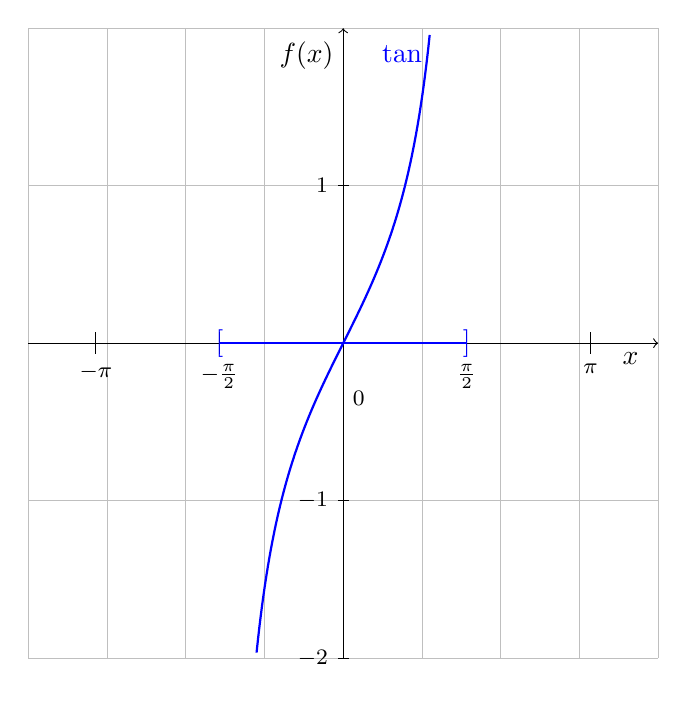
\begin{tikzpicture}[xscale=1,yscale=2]
	
	% Gitternetzlinien
	\draw[xstep=1cm, ystep=1cm, very thin, color=lightgray] (-4,2) grid (4,-2);
	% x-Achse
	\draw[->] (-4,0) -- (4,0) node[below,xshift=-1em] {$x$}; 
	%Zahlen auf x-Achse
	\foreach \x in {-3.14,-3.14/2}
	\draw[shift={(\x,0)},color=black] (0pt,2pt) -- (0pt,-2pt);
	\foreach \x in {3.14/2,3.14}
	\draw[shift={(\x,0)},color=black] (0pt,2pt) -- (0pt,-2pt);
	% y-Achse 
	\draw[->] (0,-2) -- (0,2) node[left,yshift=-1em] {$f(x)$};%node[above left]
	%Zahlen auf y-Achse
	\foreach \y in {-2,...,-1}
	\draw[shift={(0,\y)},color=black] (2pt,0pt) -- (-2pt,0pt) node[left] {\footnotesize $\y$};
	\foreach \y in {1,...,1}
	\draw[shift={(0,\y)},color=black] (2pt,0pt) -- (-2pt,0pt) node[left] {\footnotesize $\y$};
	%Ursprung
	\draw[color=black] (0pt,-10pt) node[right] {\footnotesize $0$};
	\draw[color=black] (3.14,-2pt) node[below] {\footnotesize $\pi$};
	%\draw[color=black] (6.28,-2pt) node[below] {\footnotesize $2\pi$};
	\draw[color=black] (1.57,-2pt) node[below] {\footnotesize $\frac{\pi}{2}$};
	\draw[color=black] (-1.57,-2pt) node[below] {\footnotesize $-\frac{\pi}{2}$};
	\draw[color=black] (-3.14,-2pt) node[below] {\footnotesize $-\pi$};
	%\draw[color=black] (3*3.14/2,-2pt) node[below] {\footnotesize $\frac{3}{2}\pi$};
	\draw[thick,color=blue] plot[samples=200, domain=-2.2/2:2.2/2] 
	(\x,{tan(\x r)}) node[below, xshift=-1em]{$\tan$};
	
	%\draw[dashed,color=black] (-3.14/2,-2)--(-3.14/2,2);
	%\draw[dashed,color=black] (3.14/2,-2)--(3.14/2,2);
	%\draw[dashed,color=black] (3.14/2+3.14,-2)--(3.14/2+3.14,2);
	\draw[color=blue,thick] (-3.14/2,0pt) node {$[$};
	\draw[color=blue,thick] (3.14/2,0pt) node { $]$};
	\draw[color=blue,thick] (-3.14/2,0)--(3.14/2,0);
	\end{tikzpicture}\\	
	Umkehrbar nur in diesen Intervall, wegen der Bijektivität.\\
	$ \tan:\;]-\frac{\pi}{2},+\frac{\pi}{2}[\;\longmapsto \mathbb{R} $\\
\end{center}
\newpage
\noindent
\begin{align*}
\arctan:=\tan^{-1}:\mathbb{R}\longmapsto\;]-\genfrac{}{}{}{1.7}{\pi}{2 },\genfrac{}{}{}{1.7}{\pi }{2}[
\end{align*}
\begin{center}
	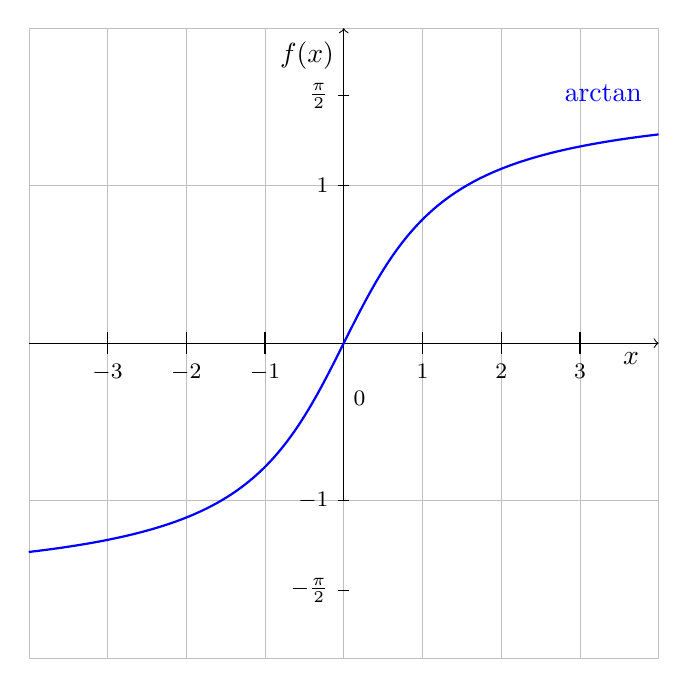
\begin{tikzpicture}[xscale=1, yscale=2]
	
	% Gitternetzlinien
	\draw[xstep=1cm, ystep=1cm, very thin, color=lightgray] (-4,2) grid (4,-2);
	% x-Achse
	\draw[->] (-4,0) -- (4,0) node[below,xshift=-1em] {$x$}; 
	%Zahlen auf x-Achse
	\foreach \x in {-3,...,-1}
	\draw[shift={(\x,0)},color=black] (0pt,2pt) -- (0pt,-2pt) node[below] {\footnotesize $\x$};
	\foreach \x in {1,...,3}
	\draw[shift={(\x,0)},color=black] (0pt,2pt) -- (0pt,-2pt) node[below] {\footnotesize $\x$};
	% y-Achse 
	\draw[->] (0,-1) -- (0,2) node[left,yshift=-1em] {$f(x)$};%node[above left]
	%Zahlen auf y-Achse
	\foreach \y in {-1,...,-1}
	\draw[shift={(0,\y)},color=black] (2pt,0pt) -- (-2pt,0pt) node[left] {\footnotesize $\y$};
	\foreach \y in {1,...,1}
	\draw[shift={(0,\y)},color=black] (2pt,0pt) -- (-2pt,0pt) node[left] {\footnotesize $\y$};
	%Ursprung
	\draw[color=black] (0pt,-10pt) node[right] {\footnotesize $0$};
	
	\draw[thick,color=blue] plot[samples=200, domain=-4:4] 
	(\x,{rad(atan(\x ))}) node[yshift=1.5em, xshift=-2em] {$\arctan$};
	
	\draw[color=black] (2pt,-3.14/2) -- (-2pt,-3.14/2) node[left] {\footnotesize $-\frac{\pi}{2}$};
	
	\draw[color=black] (2pt,3.14/2) -- (-2pt,3.14/2) node[left] {\footnotesize $\frac{\pi}{2}$};
	\end{tikzpicture}\\
\end{center}
\begin{align*}
\arctan'(x)=\frac{1}{1+x^2}
\end{align*}
$ \blacktriangleright $ Umkehrfunktion vom Kotangens.\\
\begin{center}
	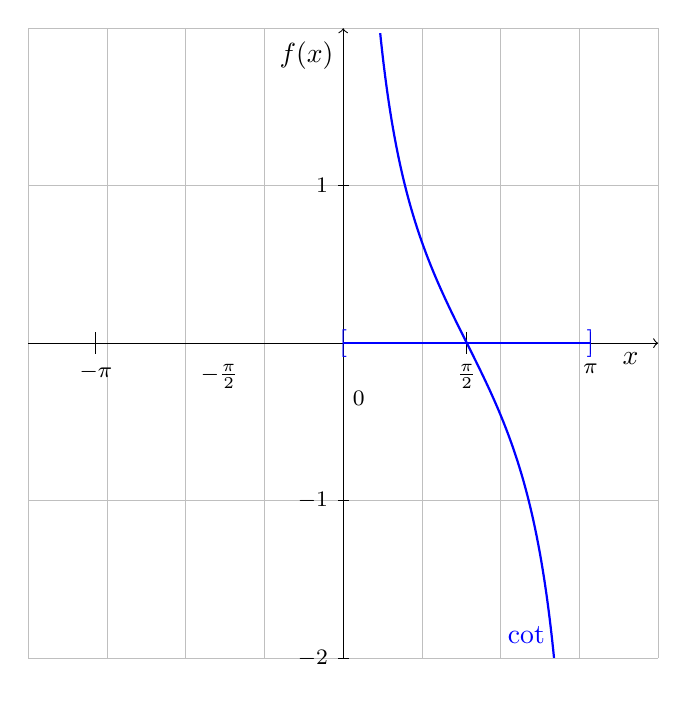
\begin{tikzpicture}[xscale=1,yscale=2]
	
	% Gitternetzlinien
	\draw[xstep=1cm, ystep=1cm, very thin, color=lightgray] (-4,2) grid (4,-2);
	% x-Achse
	\draw[->] (-4,0) -- (4,0) node[below,xshift=-1em] {$x$}; 
	%Zahlen auf x-Achse
	\foreach \x in {-3.14,3.14}
	\draw[shift={(\x,0)},color=black] (0pt,2pt) -- (0pt,-2pt);
	\foreach \x in {3.14/2,3.14}
	\draw[shift={(\x,0)},color=black] (0pt,2pt) -- (0pt,-2pt);
	% y-Achse 
	\draw[->] (0,-2) -- (0,2) node[left,yshift=-1em] {$f(x)$};%node[above left]
	%Zahlen auf y-Achse
	\foreach \y in {-2,...,-1}
	\draw[shift={(0,\y)},color=black] (2pt,0pt) -- (-2pt,0pt) node[left] {\footnotesize $\y$};
	\foreach \y in {1,...,1}
	\draw[shift={(0,\y)},color=black] (2pt,0pt) -- (-2pt,0pt) node[left] {\footnotesize $\y$};
	%Ursprung
	\draw[color=black] (0pt,-10pt) node[right] {\footnotesize $0$};
	\draw[color=black] (3.14,-2pt) node[below] {\footnotesize $\pi$};
	%\draw[color=black] (6.28,-2pt) node[below] {\footnotesize $2\pi$};
	\draw[color=black] (1.57,-2pt) node[below] {\footnotesize $\frac{\pi}{2}$};
	\draw[color=black] (-1.57,-2pt) node[below] {\footnotesize $-\frac{\pi}{2}$};
	\draw[color=black] (-3.14,-2pt) node[below] {\footnotesize $-\pi$};
	%\draw[color=black] (3*3.14/2,-2pt) node[below] {\footnotesize $\frac{3}{2}\pi$};
	\draw[thick,color=blue] plot[samples=200, domain=0.47:2.68] 
	(\x,{cot(\x r)}) node[below, xshift=-1em,yshift=15]{$\cot$};
	
	\draw[color=blue,thick] (0/2,0pt) node {$[$};
	\draw[color=blue,thick] (3.14,0pt) node { $]$};
	\draw[color=blue,thick] (0,0)--(3.14,0);
	%\draw[dashed,color=black] (-3.14,-2)--(-3.14,2);
	%\draw[dashed,color=black] (3.14,-2)--(3.14,2);
	%\draw[dashed,color=black] (3.14/2+3.14,-2)--(3.14/2+3.14,2);
	\end{tikzpicture}\\	
	Umkehrbar nur in diesen Intervall, wegen der Bijektivität.\\
	$ \cot:\;]0,\pi[\;\longmapsto\mathbb{R} $\\
\end{center}
\begin{align*}
\mathrm{arccot}:=\cot^{-1}:\mathbb{R}\longmapsto\;]0,\pi[
\end{align*}
\begin{align*}
\mathrm{arccot}'=-\frac{1}{1+x^2}
\end{align*}
\newpage
\noindent
\subsubsection{Aufgabe 1 zu trigonometrischen Funktionen}
\href{https://youtu.be/voAHLA8F08c}{Video 09}\\
Bestimme den maximalen Definitionsbereich und die Ableitung von:\\
\begin{align*}
f(x)=(\arccos(4-x))^5
\end{align*}
Es gilt:\\
\begin{align*}
&\arccos: [-1,1]\longmapsto [0,\pi]\\
&\arccos'(x)=-\frac{1}{\sqrt{1-x^2}}
\end{align*}
(i)\;\;Zum max. Definitionsbereich.\\
\begin{quote}
	\begin{align*}
	&f(x)=(\arccos(4-x))^5\\
	&\Rightarrow\\
	&\text{Für }\;\;-1\leq 4-x\leq 1\;\;\text{ist }\;\;f(x)\;\;\text{definiert. }
	\end{align*}
	D.h.:\\
	\begin{align*}
	&-1\leq 4-x\leq 1\\
	&\overset{(-4)}{\Leftrightarrow}\\
	&-5\leq -x\leq -3\\
	&\overset{(\cdot -1)}{\Leftrightarrow}\\
	&5\geq x\geq 3\\
	&\Rightarrow\mathbb{D}_f=[3,5]\\
	\end{align*}
\end{quote}
(ii)\;\;Bestimmung von $ f'(x) $.\\
\begin{quote}
	$ f(x) $ ist diffbar, weil es eine Komposition von diff. Funktionen ist.\\
	\begin{align*}
	f'(x)=(\arccos^5(4-x))'&=5\cdot \arccos^4(4-x)\cdot(\arccos(4-x))'\\
	&=5\cdot \arccos^4(4-x)\cdot\bigg(-\frac{1}{\sqrt{1-(4-x)^2}}\bigg)\cdot(4-x)'\\
	&=5\cdot \arccos^4(4-x)\cdot\frac{1}{\sqrt{1-(4-x)^2}}\\
	&=\frac{5\cdot \arccos^4(4-x)}{\sqrt{1-(4-x)^2}}\\
	\end{align*}
\end{quote}
\subsubsection{Aufgabe 2 zu trigonometrischen Funktionen}
\href{https://youtu.be/dyxaIIiA6r4}{Video 10}\\
Bestimme den maximalen Definitionsbereich von:\\
\begin{align*}
g(x)=\arcsin\bigg(\frac{1-x^2}{1+x^2}\bigg)
\end{align*}
Wenn möglich, bestimme $ g'(x) $.\\
Es gilt:\\
\begin{align*}
&\arcsin: [-1,1]\longmapsto [-\genfrac{}{}{}{1.7}{\pi }{2 },\genfrac{}{}{}{1.7}{\pi }{2 }]\\
&\arcsin'(x)=\frac{1}{\sqrt{1-x^2}}
\end{align*}
(i)\;\;Zum max. Definitionsbereich.\\
\begin{quote}
	\begin{align*}
	&g(x)=\arcsin\bigg(\frac{1-x^2}{1+x^2}\bigg)\\
	&\Rightarrow\\
	&-1\leq\frac{1-x^2}{1+x^2}\leq 1
	\end{align*}
	D.h:\\
	Für $ -1\leq\frac{1-x^2}{1+x^2} $ gilt:\\
	\begin{align*}
	&-1\leq\frac{1-x^2}{1+x^2}\\
	&\overset{(1+x^2>0)}{\Leftrightarrow}\\
	&-1(1+x^2)\leq 1-x^2\\
	&-1-x^2\leq 1-x^2\\
	&-1\leq 1\\
	&\Rightarrow \frac{1-x^2}{1+x^2}\geq -1
	\end{align*}
	Für $ 1\geq\frac{1-x^2}{1+x^2} $ gilt:\\
	\begin{align*}
	&\frac{1-x^2}{1+x^2}\leq 1\\
	&\overset{(1+x^2>0)}{\Leftrightarrow}\\
	&1-x^2\leq 1(1+x^2)\\
	&\overset{(x^2)}{\Leftrightarrow}\\
	&1\leq 1+2x^2\\
	&\Rightarrow \frac{1-x^2}{1+x^2}\leq 1
	\end{align*}	
	D.h: Maximaler Definitionsbereich ist $ \mathbb{D}_g =\mathbb{R}$\\
\end{quote}
(ii)\;\;Bestimmung von $ g'(x) $:\\
\begin{quote}
	$ g(x) $ ist diffbar, weil es eine Komposition von diff. Funktionen ist.\\
	\begin{align*}
	g'(x)=\bigg(\arcsin\bigg(\frac{1-x^2}{1+x^2}\bigg)\bigg)'&=\frac{1}{\sqrt{1-(\frac{1-x^2}{1+x^2})^2}}\cdot\bigg(\frac{1-x^2}{1+x^2}\bigg)'\\
	&=\frac{1}{\sqrt{1-(\frac{1-x^2}{1+x^2})^2}}\cdot \frac{-2x(1+x^2)-(1-x^2)2x}{(1+x^2)^2}\\
	&=\frac{1}{\sqrt{1-(\frac{1-x^2}{1+x^2})^2}}\cdot\frac{-2x-2x^2-2x+2x^2}{(1+x^2)^2}\\
	&=\frac{-4x}{\sqrt{1-(\frac{1-x^2}{1+x^2})^2}}\cdot \frac{1}{(1+x^2)^2}
	\end{align*}
\end{quote}
\subsubsection{Aufgabe 3 zu trigonometrischen Funktionen}
\href{https://youtu.be/jgmWhGejYJI}{Video 11}\\
Beweise: $ \arccos(x) +\arcsin(x)=\frac{\pi}{2} $ für $ ]-1,1[ $ .\\
\\
Definiere:\\
\begin{align*}
f(x)=\arccos(x) +\arcsin(x)
\end{align*}
Es gilt:\\
\begin{align*}
f'(x)=\frac{1}{\sqrt{1-x^2}}-\frac{1}{\sqrt{1-x^2}}=0 \;\;\text{für }\;\;x\in\;\;]-1,1[
\end{align*}
Wegen dem Konstanzkriterium gilt, dass $ f(x) $ konstant ist.\\
D.h.:\\
\begin{align*}
&f(x)=k\;\;\text{ für}\;\;k=\in\mathbb{R}\\
&f(0)=\arccos(0) +\arcsin(0)\\
&f(0)=0+\frac{\pi}{2}\\
&\Rightarrow \arccos(x) +\arcsin(x)=\frac{\pi}{2}
\end{align*}
\begin{center}
	\begin{tikzpicture}[xscale=3, yscale=2]
	
	% Gitternetzlinien
	\draw[xstep=1cm, ystep=1cm, very thin, color=lightgray] (-2,4) grid (2,-2);
	% x-Achse
	\draw[->] (-2,0) -- (2,0) node[below,xshift=-1em] {$x$}; 
	%Zahlen auf x-Achse
	\foreach \x in {-1,...,-1}
	\draw[shift={(\x,0)},color=black] (0pt,2pt) -- (0pt,-2pt) node[below] {\footnotesize $\x$};
	\foreach \x in {1,...,1}
	\draw[shift={(\x,0)},color=black] (0pt,2pt) -- (0pt,-2pt) node[below] {\footnotesize $\x$};
	% y-Achse 
	\draw[->] (0,-2) -- (0,4) node[left,yshift=-1em] {$f(x)$};%node[above left]
	%Zahlen auf y-Achse
	\foreach \y in {-1,...,-1}
	\draw[shift={(0,\y)},color=black] (2pt,0pt) -- (-2pt,0pt) node[left] {\footnotesize $\y$};
	\foreach \y in {1,...,3}
	\draw[shift={(0,\y)},color=black] (2pt,0pt) -- (-2pt,0pt) node[left] {\footnotesize $\y$};
	%Ursprung
	\draw[color=black] (0pt,-10pt) node[right] {\footnotesize $0$};
	
	\draw[thick,color=blue] plot[samples=200, domain=-0.999:0.999] 
	(\x,{rad(acos(\x ))}) node[yshift=1, xshift=2.5em] {$\arccos(x)$};
	\draw[thick,color=blue] plot[samples=200, domain=-0.999:0.999] 
	(\x,{rad(asin(\x ))}) node[yshift=1, xshift=2.5em] {$\arcsin(x)$};
	\draw[color=black] (2pt,3.14) -- (-2pt,3.14) node[left] {\footnotesize $\pi$};
	
	\draw[color=black] (2pt,3.14/2) -- (-2pt,3.14/2) node[left] {\footnotesize $\frac{\pi}{2}$};
	%		\draw[thick,color=blue] plot[samples=200, domain=-2:2] 
	%	(\x,{sinh(\x )}) node[yshift=1, xshift=2.5em] {$\arcsin(x)$};
	%	\draw[color=black] (2pt,3.14) -- (-2pt,3.14) node[left] {\footnotesize $\pi$};
	\end{tikzpicture}\\
	
	
\end{center}
\subsection{Sinus Hyperbolicus und Kosinus Hyperbolicus}
\href{https://youtu.be/FTkh0mVQCD0}{Video 12}\\
\underline{Analogie zum Cosinus und Sinus:}\\
\\
Es gilt mit eulerischer Formel: $ \mathrm{e}^{\mathrm{i}x}=\cos(x)+\mathrm{i}\cdot \sin(x) $ :\\
\begin{align*}
\frac{\mathrm{e}^{\mathrm{i}x}+\mathrm{e}^{-\mathrm{i}x}}{2}&=\frac{1}{2}\bigg[(\cos\big(x)+\mathrm{i}\cdot \sin(x)\big)+\big(\cos(-x)+\mathrm{i}\cdot \sin(-x)\big)\bigg]\\
&=\frac{1}{2}\big(\cos(x)+\mathrm{i}\cdot \sin(x)+\cos(x)-\mathrm{i}\cdot \sin(x)\big)\\
&=\frac{1}{2}(2\cdot \cos(x))\\
\frac{\mathrm{e}^{\mathrm{i}x}+\mathrm{e}^{-\mathrm{i}x}}{2}&=\cos(x)\\
\end{align*}
Analog gilt:\\
\begin{align*}
\frac{\mathrm{e}^{\mathrm{i}x}-\mathrm{e}^{-\mathrm{i}x}}{2\mathrm{i}}&=\sin(x)\\
\end{align*}
\underline {Kosinius Hyperbolikus}\\
\begin{align*}
\cosh(x)=\frac{\mathrm{e}^x+\mathrm{e}^{-x}}{2}\;\;\text{mit: } \cosh:\mathbb{R}\longmapsto[1,\infty]\\
\end{align*}
\begin{align*}
\cosh'(x)&=\bigg(\frac{\mathrm{e}^x+\mathrm{e}^{-x}}{2}\bigg)'=\frac{1}{2}\bigg[(\mathrm{e}^x)'+(\mathrm{e}^{-x})'\bigg]\\
\cosh'(x)&=\frac{\mathrm{e}^x-\mathrm{e}^{-x}}{2}=\sinh(x)
\end{align*}
Die Funktion $f(x) =\cosh(x) $ ist gerade (symmetrisch zur y-Achse),\\ weil gilt: $ f(x)=f(-x) $.\\
\begin{align*}
\cosh(-x)=\frac{\mathrm{e}^{-x}+\mathrm{e}^{-(-x)}}{2}=\frac{\mathrm{e}^x+\mathrm{e}^{-x}}{2}=\cosh(x)\\
\end{align*}
\begin{center}
	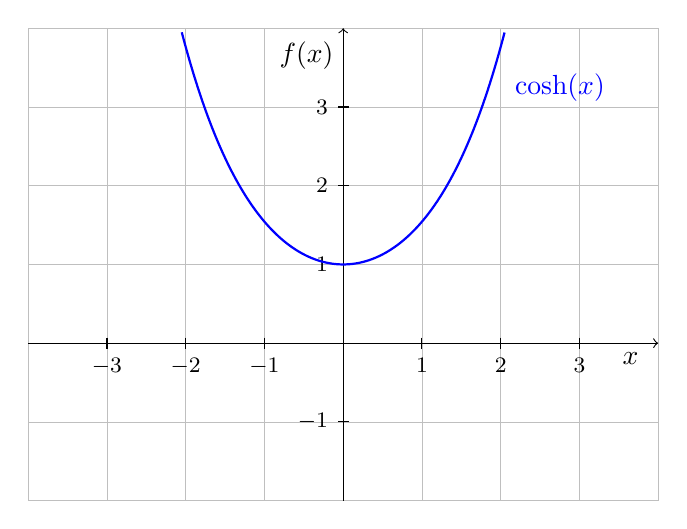
\begin{tikzpicture}[xscale=1, yscale=1]
	
	% Gitternetzlinien
	\draw[xstep=1cm, ystep=1cm, very thin, color=lightgray] (-4,4) grid (4,-2);
	% x-Achse
	\draw[->] (-4,0) -- (4,0) node[below,xshift=-1em] {$x$}; 
	%Zahlen auf x-Achse
	\foreach \x in {-3,...,-1}
	\draw[shift={(\x,0)},color=black] (0pt,2pt) -- (0pt,-2pt) node[below] {\footnotesize $\x$};
	\foreach \x in {1,...,3}
	\draw[shift={(\x,0)},color=black] (0pt,2pt) -- (0pt,-2pt) node[below] {\footnotesize $\x$};
	% y-Achse 
	\draw[->] (0,-2) -- (0,4) node[left,yshift=-1em] {$f(x)$};%node[above left]
	%Zahlen auf y-Achse
	\foreach \y in {-1,...,-1}
	\draw[shift={(0,\y)},color=black] (2pt,0pt) -- (-2pt,0pt) node[left] {\footnotesize $\y$};
	\foreach \y in {1,...,3}
	\draw[shift={(0,\y)},color=black] (2pt,0pt) -- (-2pt,0pt) node[left] {\footnotesize $\y$};
	%Ursprung
	
	
	
	\draw[thick,color=blue] plot[samples=200, domain=-2.05:2.05] 
	(\x,{cosh(\x )}) node[yshift=-2em, xshift=2em] {$\cosh(x)$};
	
	
	\end{tikzpicture}\\
	
\end{center}
\underline{Sinus Hyperbolikus}
\begin{align*}
\sinh(x)=\frac{\mathrm{e}^x-\mathrm{e}^{-x}}{2}\;\;\text{mit: } \sinh:\mathbb{R}\longmapsto\mathbb{R}\\
\end{align*}
\begin{align*}
\sinh'(x)&=\bigg(\frac{\mathrm{e}^x-\mathrm{e}^{-x}}{2}\bigg)'=\frac{1}{2}\bigg[(\mathrm{e}^x)'-(\mathrm{e}^{-x})'\bigg]\\
\sinh'(x)&=\frac{\mathrm{e}^x+\mathrm{e}^{-x}}{2}=\cosh(x)
\end{align*}
Die Funktion $f(x) =\sinh(x) $ ist ungerade (Punktsymmetrisch zum Nullpunkt),\\ weil gilt: $ f(-x)=-f(x) $.\\
\begin{align*}
\sinh(-x)=\frac{\mathrm{e}^{-x}-\mathrm{e}^x}{2}=\frac{-\mathrm{e}^x+\mathrm{e}^{-x}}{2}=-\bigg(\frac{\mathrm{e}^x-\mathrm{e}^{-x}}{2}\bigg)=-\sinh(x)
\end{align*}
\begin{center}
	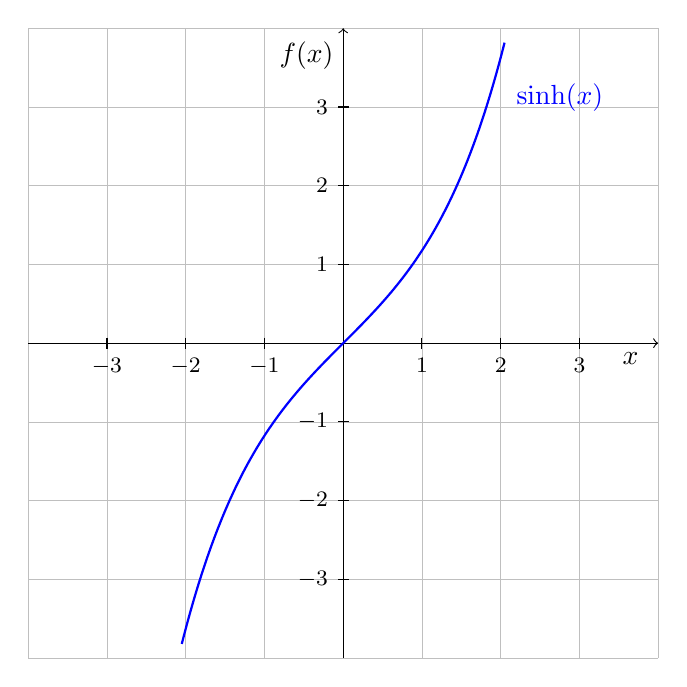
\begin{tikzpicture}[xscale=1, yscale=1]
	
	% Gitternetzlinien
	\draw[xstep=1cm, ystep=1cm, very thin, color=lightgray] (-4,4) grid (4,-4);
	% x-Achse
	\draw[->] (-4,0) -- (4,0) node[below,xshift=-1em] {$x$}; 
	%Zahlen auf x-Achse
	\foreach \x in {-3,...,-1}
	\draw[shift={(\x,0)},color=black] (0pt,2pt) -- (0pt,-2pt) node[below] {\footnotesize $\x$};
	\foreach \x in {1,...,3}
	\draw[shift={(\x,0)},color=black] (0pt,2pt) -- (0pt,-2pt) node[below] {\footnotesize $\x$};
	% y-Achse 
	\draw[->] (0,-4) -- (0,4) node[left,yshift=-1em] {$f(x)$};%node[above left]
	%Zahlen auf y-Achse
	\foreach \y in {-3,...,-1}
	\draw[shift={(0,\y)},color=black] (2pt,0pt) -- (-2pt,0pt) node[left] {\footnotesize $\y$};
	\foreach \y in {1,...,3}
	\draw[shift={(0,\y)},color=black] (2pt,0pt) -- (-2pt,0pt) node[left] {\footnotesize $\y$};
	%Ursprung
	
	
	
	\draw[thick,color=blue] plot[samples=200, domain=-2.05:2.05] 
	(\x,{sinh(\x )}) node[yshift=-2em, xshift=2em] {$\sinh(x)$};
	
	
	
	\end{tikzpicture}\\
	
\end{center}
\underline{Hyperbelgleichung}
\begin{align*}
\cosh^2(x)-\sinh^2(x)=1
\end{align*}
Beweis:\\
\begin{align*}
\cosh^2(x)-\sinh^2(x)&=\bigg(\frac{\mathrm{e}^x+\mathrm{e}^{-x}}{2}\bigg)^2-\bigg(\frac{\mathrm{e}^x-\mathrm{e}^{-x}}{2}\bigg)^2\\
&=\bigg(\frac{1}{2}\bigg)^2\bigg[(\mathrm{e}^x+\mathrm{e}^{-x})^2-(\mathrm{e}^x-\mathrm{e}^{-x})^2\bigg]\\
&=\frac{1}{4}\cdot \bigg[\mathrm{e}^{2x}+\underbrace {2\mathrm{e}^x\mathrm{e}^{-x}}_{=2}+\mathrm{e}^{-2x}-(\mathrm{e}^{2x}-\underbrace {2\mathrm{e}^x\mathrm{e}^{-x}}_{=-2}+\mathrm{e}^{-2x})\bigg]\\
&=\frac{1}{4}(2+2)=1_{_{\Square}}
\end{align*}
\underline{Einheitshyperbel}\\
Für die gilt:\\
\begin{align*}
\{(x,y)|x^2-y^2=1\}
\end{align*}
Der Kosinus Hyperbolikus und der Sinus Hyperolikus sind auf der Einheitshyperbel.\\
\begin{center}
	
	
	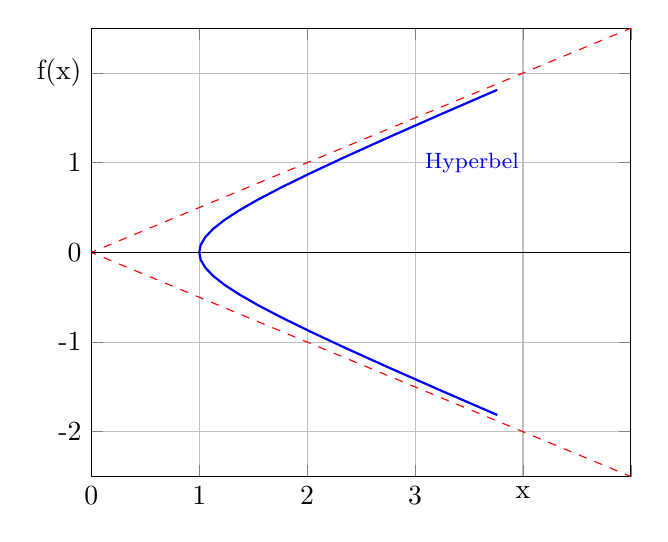
\begin{tikzpicture}
	
	\begin{axis}[grid = major,xticklabels={0,0,1,2,3,{x}},yticklabels={0,-2,-1,0,1,{f(x)}},
	%ylabel near ticks,
	%xlabel = {x},
	%xlabel = {x},
	%ylabel = {y},
	xmin=0,xmax=5,
	ymin=-5,ymax=5]
	\node[blue,right] at (axis cs:3,2) {\footnotesize Hyperbel };
	\addplot [blue,thick,domain=-2:2] ({cosh(x)}, {sinh(x)});
	\addplot[red,dashed] expression {x};
	\addplot[red,dashed] expression {-x};
	\addplot[black] expression {0};
	\draw[blue,thick] ({axis cs:6,1}) node[above,right] {Formel 2};
	
	\end{axis}
	\end{tikzpicture}
\end{center}
\underline{Einheitskreis}\\
Für den gilt wegen:
\begin{align*}
\cos^2(x)+\sin^2(x)=1 \\
\end{align*}
\begin{align*}
\{(x,y)|x^2+y^2=1\}
\end{align*}
\begin{center}
	
	
	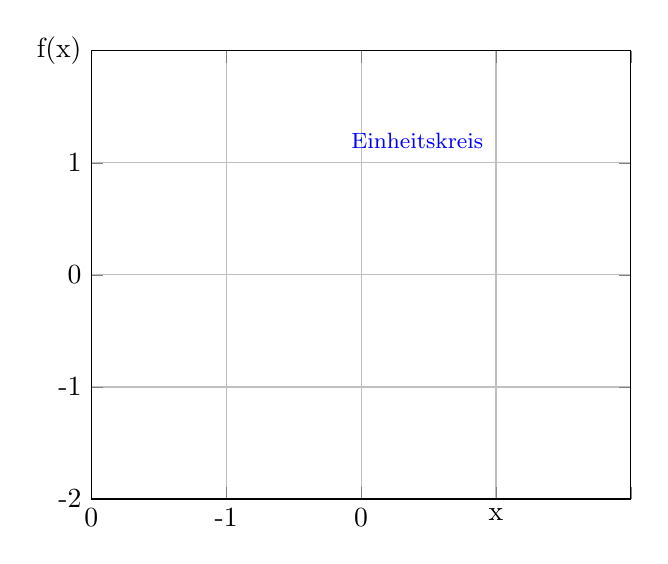
\begin{tikzpicture}
	
	\begin{axis}[grid = major,
	%ylabel near ticks,
	%xlabel = {x},
	%xlabel = {x},
	%ylabel = {y},
	xmin=-2,xmax=2,
	ymin=-2,ymax=2,xticklabels={0,0,-1,0,{x}},yticklabels={0,-2,-1,0,1,{f(x)}},]
	\node[blue,left of=eft] at (axis cs:1,1.2) {\footnotesize Einheitskreis };
	
	
	
	\draw[blue, thick] (axis cs:0,0) circle (100);
	
	
	\end{axis}
	\end{tikzpicture}
\end{center}
Der Sinus und der Cosinus sind auf dem Einheitskreis.\\
Bemerkung:\\
Der Sinus Hyperbolikus und der Kosinus Hyperbolikus sind der ungerade und gerade Anteil der Exponentialfunktion.\\
\begin{align*}
\mathrm{e}^x=\cosh(x)+\sinh(x)=\frac{\mathrm{e}^{x}}{2}+\frac{\mathrm{e}^{-x}}{2}+\frac{\mathrm{e}^{x}}{2}-\frac{\mathrm{e}^{-x}}{2}=\mathrm{e}^x\\
\end{align*}
\subsubsection{Tangens Hyperbolicus}
\href{https://youtu.be/cUg7vCA_ggw}{Video 13}\\
Es gilt für den Tangens:\\
\begin{align*}
\tan(x)=\frac{\sin(x)}{\cos(x)}
\end{align*}
Analog gilt für den Tangens Hyperbolikus:\\
\begin{align*}
\tanh(x)=\frac{\sinh(x)}{\cosh(x)}=\frac{\mathrm{e}^x-\mathrm{e}^{-x}}{\mathrm{e}^x+\mathrm{e}^{-x}}\;\;\text{mit }\;\;\tanh:\mathbb{R}\longmapsto\; ]-1,1[
\end{align*}
\newpage
\noindent
Warum gilt: $\tanh:\mathbb{R}\longmapsto\; ]-1,1[  $ ?
\begin{quote}
	\textbullet\;\;Es gilt: \\
	\begin{align*}
	&\frac{\mathrm{e}^x-\mathrm{e}^{-x}}{\mathrm{e}^x+\mathrm{e}^{-x}}\overset{!}{<}1\\
	&\mathrm{e}^x-\mathrm{e}^{-x}<\mathrm{e}^x+\mathrm{e}^{-x}\boxed{}\;\;\text{ $ \mathrm{e}^x $ ist immer positiv}\\
	&\Rightarrow\\
	&\mathrm{e}^x-\mathrm{e}^{-x}\neq\mathrm{e}^x+\mathrm{e}^{-x}\\
	&\Rightarrow\\
	&\frac{\mathrm{e}^x-\mathrm{e}^{-x}}{\mathrm{e}^x+\mathrm{e}^{-x}}<1
	\end{align*}
	\textbullet \;\;Ebenso gilt:\\
	\begin{align*}
	&\frac{\mathrm{e}^x-\mathrm{e}^{-x}}{\mathrm{e}^x+\mathrm{e}^{-x}}\overset{!}{>}-1\\
	&\mathrm{e}^x-\mathrm{e}^{-x}>-1(\mathrm{e}^x+\mathrm{e}^{-x})\\
	&\mathrm{e}^x-\mathrm{e}^{-x}>-\mathrm{e}^x-\mathrm{e}^{-x}\boxed{}\\
	&\Rightarrow\\
	&\mathrm{e}^x-\mathrm{e}^{-x}\neq-1(\mathrm{e}^x+\mathrm{e}^{-x})\\
	&\Rightarrow\\
	&\frac{\mathrm{e}^x-\mathrm{e}^{-x}}{\mathrm{e}^x+\mathrm{e}^{-x}}>-1
	\end{align*}
	\begin{align*}
	\Rightarrow \tanh:\mathbb{R}\longmapsto\; ]-1,1[
	\end{align*}
	
	
	
\end{quote}
Ableitung vom Tangens Hyperbolikus:\\
\begin{align*}
\tanh'(x)=\bigg(\tanh(x)=\frac{\sinh(x)}{\cosh(x)}\bigg)'=\frac{\cosh^2(x)-\sinh^2(x)}{\cosh^2(x)}=1-\frac{\sinh^2(x)}{\cosh^2(x)}\\
\end{align*}
\begin{quote}
	Ebenso gilt:\\
	\begin{align*}
	\cosh^2(x)-\sinh^2(x)=1
	\end{align*}
	Also gilt:\\
	\begin{align*}
	\tanh'(x)=\frac{1}{\cosh^2(x)}=1-\frac{\sinh^2(x)}{\cosh^2(x)}=1-\tanh^2(x)\\
	\end{align*}
\end{quote}

\begin{center}
	\begin{tikzpicture}[xscale=3, yscale=2]
	
	% Gitternetzlinien
	\draw[xstep=1cm, ystep=1cm, very thin, color=lightgray] (-2,2) grid (2,-2);
	% x-Achse
	\draw[->] (-2,0) -- (2,0) node[below,xshift=-1em] {$x$}; 
	%Zahlen auf x-Achse
	\foreach \x in {-1,...,-1}
	\draw[shift={(\x,0)},color=black] (0pt,2pt) -- (0pt,-2pt) node[below] {\footnotesize $\x$};
	\foreach \x in {1,...,1}
	\draw[shift={(\x,0)},color=black] (0pt,2pt) -- (0pt,-2pt) node[below] {\footnotesize $\x$};
	% y-Achse 
	\draw[->] (0,-2) -- (0,2) node[left,yshift=-1em] {$f(x)$};%node[above left]
	%Zahlen auf y-Achse
	\foreach \y in {-1,...,-1}
	\draw[shift={(0,\y)},color=black] (2pt,0pt) -- (-2pt,0pt) node[left] {\footnotesize $\y$};
	\foreach \y in {1,...,2}
	\draw[shift={(0,\y)},color=black] (2pt,0pt) -- (-2pt,0pt) node[left] {\footnotesize $\y$};
	%Ursprung
	\draw[color=black] (0pt,-10pt) node[right] {\footnotesize $0$};
	\draw[thick,color=blue] plot[samples=200, domain=-2.0:2.0] 
	(\x,{tanh(\x )}) node[yshift=-2em, xshift=-2em] {$\tanh(x)$};
	\draw[color=blue,dashed] (-2,1)--(2,1);
	\draw[color=blue,dashed] (-2,-1)--(2,-1);
	%		\draw[thick,color=blue] plot[samples=200, domain=-2:2] 
	%	(\x,{sinh(\x )}) node[yshift=1, xshift=2.5em] {$\arcsin(x)$};
	%	\draw[color=black] (2pt,3.14) -- (-2pt,3.14) node[left] {\footnotesize $\pi$};
	\end{tikzpicture}\\
	
	
\end{center}
Der Tangens Hyperbolikus ist streng monoton wachsend wegen $ \tanh'(x)=\frac{1}{\cosh^2(x)}>0 $.\\
\subsubsection{Kotangens Hyperbolicus}
\href{https://youtu.be/4mRuIkIRMCY}{Video 14}\\
Es gilt für den Kotangens:\\
\begin{align*}
\cot(x)=\frac{\cos(x)}{\sin(x)}
\end{align*}
Analog gilt für den Kotangens Hyperbolikus:\\
\begin{align*}
\coth(x)=\frac{\cosh(x)}{\sinh(x)}=\frac{\mathrm{e}^x+\mathrm{e}^{-x}}{\mathrm{e}^x-\mathrm{e}^{-x}}\;\;\text{mit }\;\;\coth:\mathbb{R}\backslash\{0\}\longmapsto \mathbb{R}\backslash \{-1,1\}
\end{align*} 
Warum gilt: $\coth:\mathbb{R}\backslash\{0\}\longmapsto \mathbb{R}\backslash \{-1,1\}  $ ?\\
\begin{quote}
	\textbullet \;\;$ \mathbb{R} \backslash\{0\}$ weil $ \mathrm{e}^x-\mathrm{e}^{-x}\neq 0 $ sein muß.\\
	\newpage
	\noindent
	\textbullet \;\; Es gilt:\\
	\begin{align*}
	&|\mathrm{e}^x-\mathrm{e}^{-x}|<|\mathrm{e}^x +\mathrm{e}^{-x}|\\
	&\Leftrightarrow\\
	&1<\bigg|\frac{\mathrm{e}^x +\mathrm{e}^{-x}}{\mathrm{e}^x-\mathrm{e}^{-x}}\bigg|\;\;\;\;|\text{\tiny $\mathrm{e}^x +\mathrm{e}^{-x}  $  immer positv }\\
	&1<\frac{\mathrm{e}^x +\mathrm{e}^{-x}}{|\mathrm{e}^x-\mathrm{e}^{-x}|}\\
	&\text{Für }\;\;\mathrm{e}^x-\mathrm{e}^{-x}<0\;\;\text{gilt: }\\
	&1<\frac{\mathrm{e}^x+\mathrm{e}^{-x}}{-(\mathrm{e}^x-\mathrm{e}^{-x})}\\
	&-1>\frac{\mathrm{e}^x+\mathrm{e}^{-x}}{\mathrm{e}^x-\mathrm{e}^{-x}}=\coth(x)\\
	&\text{Für }\;\;\mathrm{e}^x-\mathrm{e}^{-x}>0\;\;\text{gilt: }\\
	&1<\frac{\mathrm{e}^x+\mathrm{e}^{-x}}{\mathrm{e}^x-\mathrm{e}^{-x}}=\coth(x)\\
	&\Rightarrow\\
	&\coth(x)>1 \wedge \coth<-1\\
	&\Rightarrow\\
	&\coth:\mathbb{R}\backslash\{0\}\longmapsto \mathbb{R}\backslash [-1,1 ]
	\end{align*}
\end{quote}
Ableitung vom Kotangens Hyperbolikus:
\begin{align*}
\coth'(x)&=\bigg(\frac{\coth(x)}{\sinh(x)}\bigg)'=\frac{\sinh^2(x)-\cosh^2(x)}{\sinh^2(x)}=1-\coth^2(x)\\
&=\frac{-(-\sinh^2(x)+\cosh^2(x))}{\sinh^2(x)}\\
&=\frac{-(\cosh^2(x)-\sinh^2(x))}{\sinh^2(x)}=-\frac{1}{\sinh^2(x)}<0
\end{align*}
D.h. der Kotangens Hyperbolikus ist streng monoton fallend in den Intervallen $ ]-\infty,0[ $ und  $ ]0,\infty[ $. \\
Für die Monotoniebetrachtung muß jedes einzelne Intervall betrachtet werden.\\
\begin{center}
	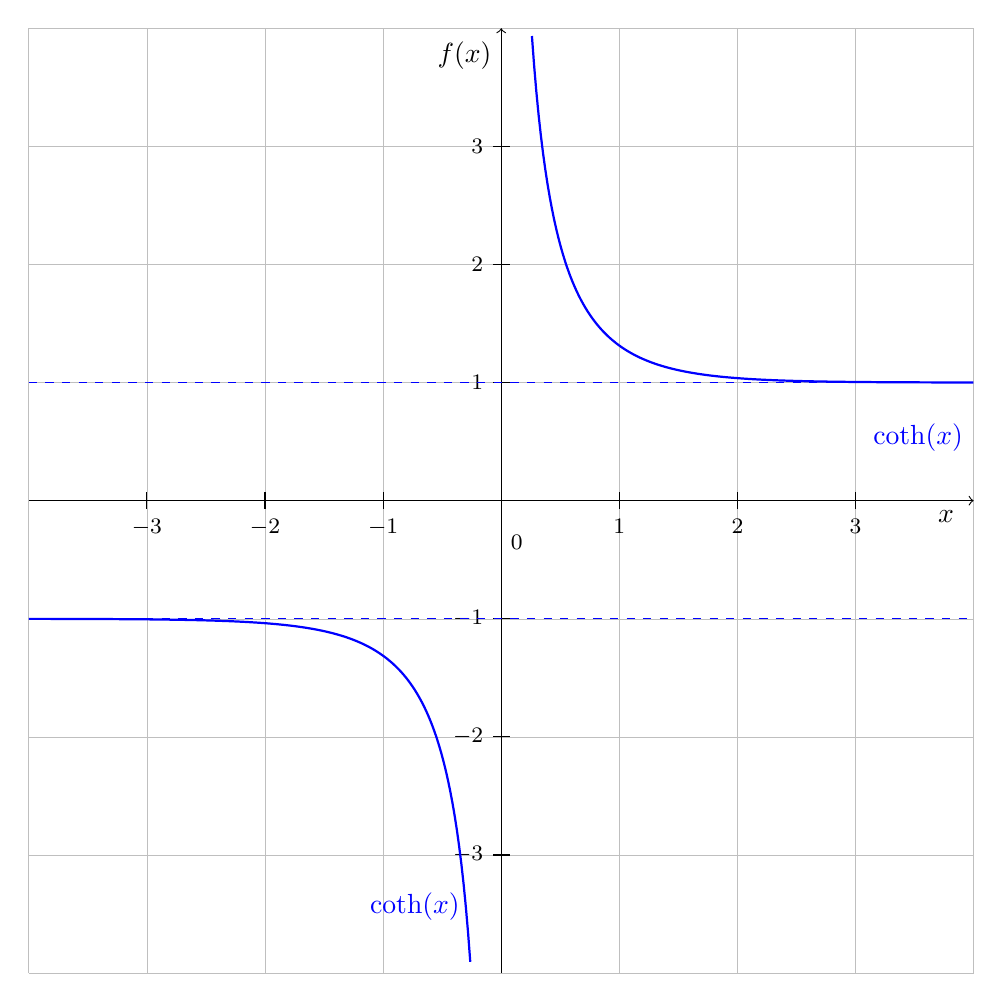
\begin{tikzpicture}[xscale=1.5, yscale=1.5]
	
	% Gitternetzlinien
	\draw[xstep=1cm, ystep=1cm, very thin, color=lightgray] (-4,4) grid (4,-4);
	% x-Achse
	\draw[->] (-4,0) -- (4,0) node[below,xshift=-1em] {$x$}; 
	%Zahlen auf x-Achse
	\foreach \x in {-3,...,-1}
	\draw[shift={(\x,0)},color=black] (0pt,2pt) -- (0pt,-2pt) node[below] {\footnotesize $\x$};
	\foreach \x in {1,...,3}
	\draw[shift={(\x,0)},color=black] (0pt,2pt) -- (0pt,-2pt) node[below] {\footnotesize $\x$};
	% y-Achse 
	\draw[->] (0,-4) -- (0,4) node[left,yshift=-1em] {$f(x)$};%node[above left]
	%Zahlen auf y-Achse
	\foreach \y in {-3,...,-1}
	\draw[shift={(0,\y)},color=black] (2pt,0pt) -- (-2pt,0pt) node[left] {\footnotesize $\y$};
	\foreach \y in {1,...,3}
	\draw[shift={(0,\y)},color=black] (2pt,0pt) -- (-2pt,0pt) node[left] {\footnotesize $\y$};
	%Ursprung
	\draw[color=black] (0pt,-10pt) node[right] {\footnotesize $0$};
	\draw[thick,color=blue] plot[samples=200, domain=-4.0:-.26] 
	(\x,{cosh(\x )/sinh(\x)}) node[yshift=2em, xshift=-2em] {$\coth(x)$};
	\draw[thick,color=blue] plot[samples=200, domain=.26:4] 
	(\x,{cosh(\x )/sinh(\x)}) node[yshift=-2em, xshift=-2em] {$\coth(x)$};
	
	\draw[color=blue,dashed] (-4,1)--(4,1);
	\draw[color=blue,dashed] (-4,-1)--(4,-1);
	
	
	%		\draw[thick,color=blue] plot[samples=200, domain=-2:2] 
	%	(\x,{sinh(\x )}) node[yshift=1, xshift=2.5em] {$\arcsin(x)$};
	%	\draw[color=black] (2pt,3.14) -- (-2pt,3.14) node[left] {\footnotesize $\pi$};
	\end{tikzpicture}\\
	
	
\end{center}
Der Kotangens Hyperbolikus ist punktsymmetrisch.\\
Es gilt für Punktsymmetrie:\\
\begin{align*}
f(-x)=-f(x)\\
\end{align*}
\begin{align*}
\coth(-x)=\frac{\cosh(-x)}{\sinh(-x)}=\frac{\cosh(x)}{-\sinh(x)}=-\coth(x)
\end{align*}
\subsubsection{Areasinus Hyperbolicus und Areakosinus Hyperbolicus}
\href{https://youtu.be/LC1HLiQZvc8}{Video 15}\\
Die Area-Funktionen sind die Umkehrfunktionen der Hyperbelfunktionen.\\
$\blacktriangleright$ Umkehrfunktion vom Kosinus Hyperbolikus.
\begin{center}
	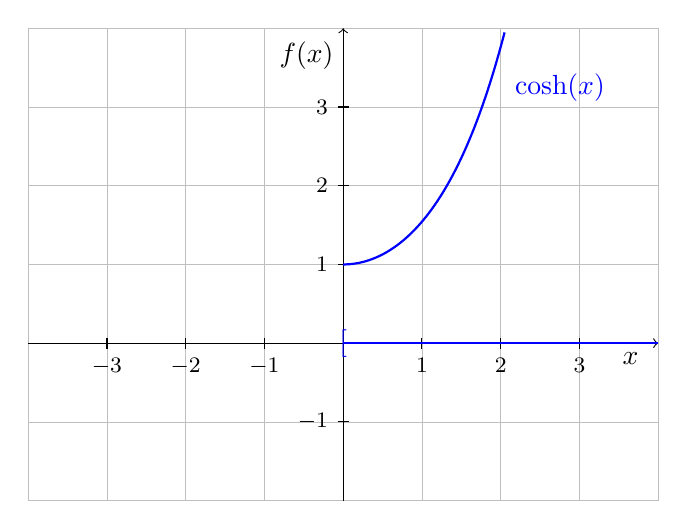
\begin{tikzpicture}[xscale=1, yscale=1]
	
	% Gitternetzlinien
	\draw[xstep=1cm, ystep=1cm, very thin, color=lightgray] (-4,4) grid (4,-2);
	% x-Achse
	\draw[->] (-4,0) -- (4,0) node[below,xshift=-1em] {$x$}; 
	%Zahlen auf x-Achse
	\foreach \x in {-3,...,-1}
	\draw[shift={(\x,0)},color=black] (0pt,2pt) -- (0pt,-2pt) node[below] {\footnotesize $\x$};
	\foreach \x in {1,...,3}
	\draw[shift={(\x,0)},color=black] (0pt,2pt) -- (0pt,-2pt) node[below] {\footnotesize $\x$};
	% y-Achse 
	\draw[->] (0,-2) -- (0,4) node[left,yshift=-1em] {$f(x)$};%node[above left]
	%Zahlen auf y-Achse
	\foreach \y in {-1,...,-1}
	\draw[shift={(0,\y)},color=black] (2pt,0pt) -- (-2pt,0pt) node[left] {\footnotesize $\y$};
	\foreach \y in {1,...,3}
	\draw[shift={(0,\y)},color=black] (2pt,0pt) -- (-2pt,0pt) node[left] {\footnotesize $\y$};
	%Ursprung
	
	
	
	\draw[thick,color=blue] plot[samples=200, domain=0:2.05] 
	(\x,{cosh(\x )}) node[yshift=-2em, xshift=2em] {$\cosh(x)$};
	\draw[color=blue,thick] (0pt,0pt) node {$[$};
	%\draw[color=blue,thick] (3.14,0pt) node { $]$};
	\draw[color=blue,thick] (0,0pt)--(4,0);
	
	\end{tikzpicture}\\
	Umkehrbahr nur in diesen Intervall, wegen der Bijektivität \\
	$\cosh:[0,\infty]\longmapsto[1,\infty] $\\ 
\end{center}
\begin{align*}
&\mathrm{arcosh}: [1,\infty[ \;\longmapsto [0,\infty[\\
&x \longmapsto \cosh^{-1}(x)=\mathrm{arcosh(x)}
\end{align*}
\begin{center}
	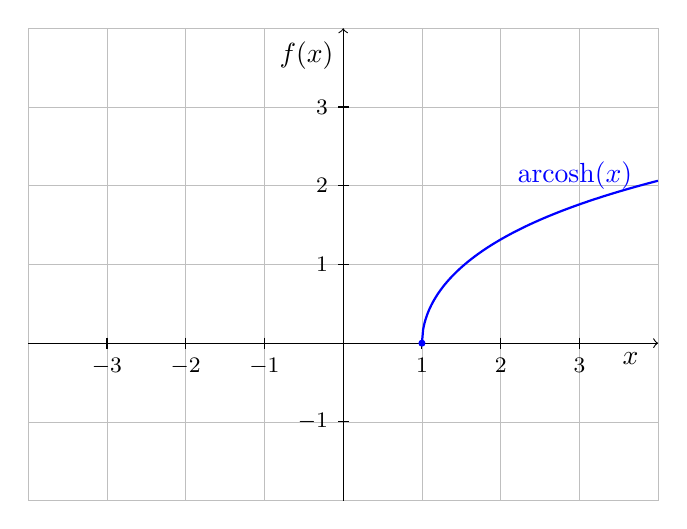
\begin{tikzpicture}[xscale=1, yscale=1]
	
	% Gitternetzlinien
	\draw[xstep=1cm, ystep=1cm, very thin, color=lightgray] (-4,4) grid (4,-2);
	% x-Achse
	\draw[->] (-4,0) -- (4,0) node[below,xshift=-1em] {$x$}; 
	%Zahlen auf x-Achse
	\foreach \x in {-3,...,-1}
	\draw[shift={(\x,0)},color=black] (0pt,2pt) -- (0pt,-2pt) node[below] {\footnotesize $\x$};
	\foreach \x in {1,...,3}
	\draw[shift={(\x,0)},color=black] (0pt,2pt) -- (0pt,-2pt) node[below] {\footnotesize $\x$};
	% y-Achse 
	\draw[->] (0,-2) -- (0,4) node[left,yshift=-1em] {$f(x)$};%node[above left]
	%Zahlen auf y-Achse
	\foreach \y in {-1,...,-1}
	\draw[shift={(0,\y)},color=black] (2pt,0pt) -- (-2pt,0pt) node[left] {\footnotesize $\y$};
	\foreach \y in {1,...,3}
	\draw[shift={(0,\y)},color=black] (2pt,0pt) -- (-2pt,0pt) node[left] {\footnotesize $\y$};
	%Ursprung
	\draw[thick,color=blue] plot[samples=200, domain=1.0:4] 
	(\x,{(ln(\x+sqrt(\x*\x-1) ))}) node[yshift=2, xshift=-3em] {$\mathrm{arcosh}(x)$};
	\fill[blue] (1,0) circle (0.045);
	
	%\draw[thick,color=blue] plot[samples=200, domain=0:2.05] 
	%	(\x,{cosh(\x )}) node[yshift=-2em, xshift=2em] {$\cosh(x)$};
	%	\draw[color=blue,thick] (0pt,0pt) node {$[$};
	%\draw[color=blue,thick] (3.14,0pt) node { $]$};
	%	\draw[color=blue,thick] (0,0pt)--(4,0);
	
	\end{tikzpicture}\\
	Umkehrbahr nur in diesen Intervall, wegen der Bijektivität \\
	$\cosh:[0,\infty]\longmapsto[1,\infty] $\\ 
\end{center}
Ableitung von Areakosinus Hyperbolikus.\\
\begin{align*}
\mathrm{arcosh}'(x)=\frac{1}{\sqrt{x^2-1}}
\end{align*}
Analog zum Arcuskosinus.\\
\begin{align*}
\arccos'(x)=\frac{-1}{\sqrt{1-x^2}}
\end{align*}
$\blacktriangleright$ Umkehrfunktion vom Sinus Hyperbolikus.
\begin{center}
	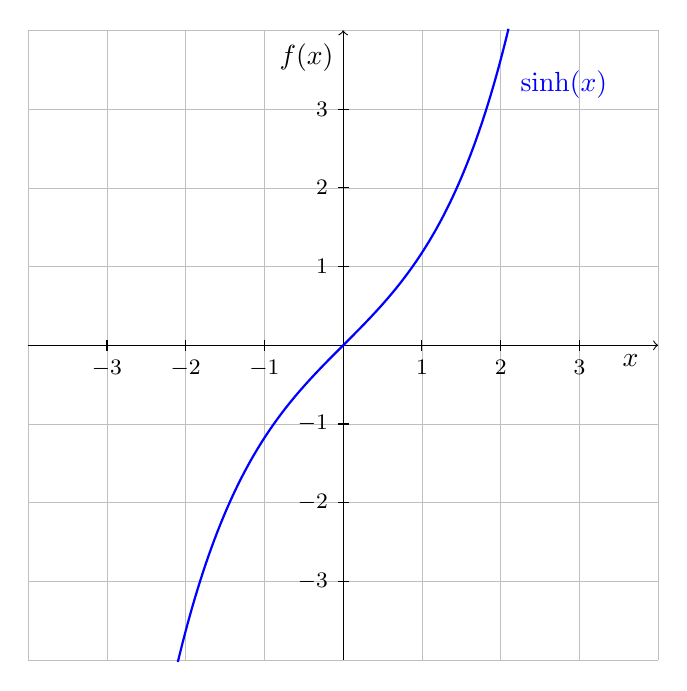
\begin{tikzpicture}[xscale=1, yscale=1]
	
	% Gitternetzlinien
	\draw[xstep=1cm, ystep=1cm, very thin, color=lightgray] (-4,4) grid (4,-4);
	% x-Achse
	\draw[->] (-4,0) -- (4,0) node[below,xshift=-1em] {$x$}; 
	%Zahlen auf x-Achse
	\foreach \x in {-3,...,-1}
	\draw[shift={(\x,0)},color=black] (0pt,2pt) -- (0pt,-2pt) node[below] {\footnotesize $\x$};
	\foreach \x in {1,...,3}
	\draw[shift={(\x,0)},color=black] (0pt,2pt) -- (0pt,-2pt) node[below] {\footnotesize $\x$};
	% y-Achse 
	\draw[->] (0,-4) -- (0,4) node[left,yshift=-1em] {$f(x)$};%node[above left]
	%Zahlen auf y-Achse
	\foreach \y in {-3,...,-1}
	\draw[shift={(0,\y)},color=black] (2pt,0pt) -- (-2pt,0pt) node[left] {\footnotesize $\y$};
	\foreach \y in {1,...,3}
	\draw[shift={(0,\y)},color=black] (2pt,0pt) -- (-2pt,0pt) node[left] {\footnotesize $\y$};
	%Ursprung
	
	
	
	\draw[thick,color=blue] plot[samples=200, domain=-2.1:2.1] 
	(\x,{sinh(\x )}) node[yshift=-2em, xshift=2em] {$\sinh(x)$};
	%\draw[color=blue,thick] (0pt,0pt) node {$[$};
	%\draw[color=blue,thick] (3.14,0pt) node { $]$};
	%\draw[color=blue,thick] (0,0pt)--(4,0);
	
	\end{tikzpicture}\\
	Umkehrbahr im ganzen Intervall. \\
	$\sinh:\mathbb{R}\longmapsto \mathbb{R}$\\ 
\end{center}
\begin{align*}
&\mathrm{arsinh: \mathbb{R}\longmapsto \mathbb{R}}\\
&x\longmapsto \sinh^{-1}(x)=\mathrm{arsinh(x)}
\end{align*}
\begin{center}
	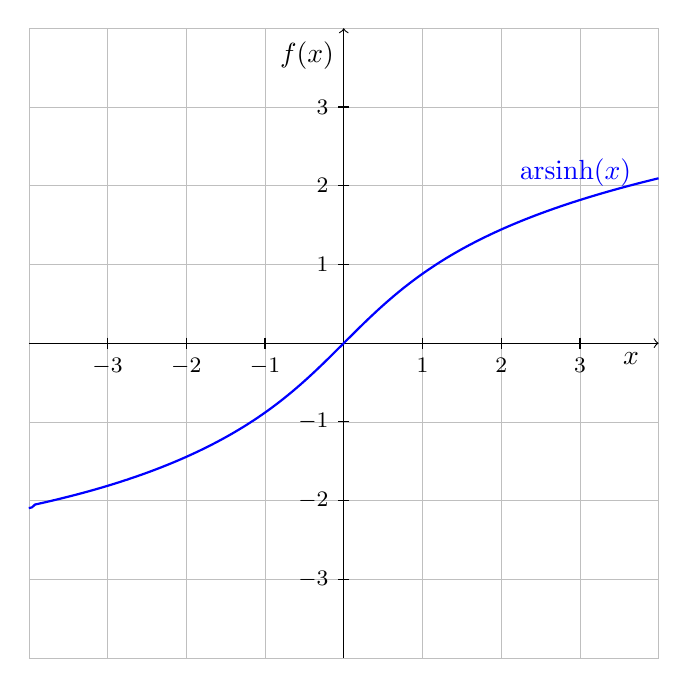
\begin{tikzpicture}[xscale=1, yscale=1]
	
	% Gitternetzlinien
	\draw[xstep=1cm, ystep=1cm, very thin, color=lightgray] (-4,4) grid (4,-4);
	% x-Achse
	\draw[->] (-4,0) -- (4,0) node[below,xshift=-1em] {$x$}; 
	%Zahlen auf x-Achse
	\foreach \x in {-3,...,-1}
	\draw[shift={(\x,0)},color=black] (0pt,2pt) -- (0pt,-2pt) node[below] {\footnotesize $\x$};
	\foreach \x in {1,...,3}
	\draw[shift={(\x,0)},color=black] (0pt,2pt) -- (0pt,-2pt) node[below] {\footnotesize $\x$};
	% y-Achse 
	\draw[->] (0,-4) -- (0,4) node[left,yshift=-1em] {$f(x)$};%node[above left]
	%Zahlen auf y-Achse
	\foreach \y in {-3,...,-1}
	\draw[shift={(0,\y)},color=black] (2pt,0pt) -- (-2pt,0pt) node[left] {\footnotesize $\y$};
	\foreach \y in {1,...,3}
	\draw[shift={(0,\y)},color=black] (2pt,0pt) -- (-2pt,0pt) node[left] {\footnotesize $\y$};
	%Ursprung
	
	\draw[thick,color=blue] plot[samples=200, domain=-4:4] 
	(\x,{(ln(\x+sqrt(\x*\x+1) ))}) node[yshift=2, xshift=-3em] {$\mathrm{arsinh}(x)$};
	%\draw[color=blue,thick] (0pt,0pt) node {$[$};
	%\draw[color=blue,thick] (3.14,0pt) node { $]$};
	%\draw[color=blue,thick] (0,0pt)--(4,0);
	
	\end{tikzpicture}\\
	
\end{center}
Ableitung von Areasinus Hyperbolikus.\\
\begin{align*}
\mathrm{arsinh}'(x)=\frac{1}{\sqrt{x^2+1}}
\end{align*}
Analog zum Arcussinus.\\
\begin{align*}
\arcsin'(x)=\frac{1}{\sqrt{1-x^2}}
\end{align*}
\subsubsection{ Areatangens Hyperbolicus und Areakotangens Hyperbolicus}
\href{https://youtu.be/B5OvQbfafVQ}{Video 16}\\
$\blacktriangleright$ Die Umkehrfunktion von Tangens Hyperbolikus ist der Areatangens Hyperbolikus.\\
\begin{center}
	\begin{tikzpicture}[xscale=3, yscale=2]
	
	% Gitternetzlinien
	\draw[xstep=1cm, ystep=1cm, very thin, color=lightgray] (-2,2) grid (2,-2);
	% x-Achse
	\draw[->] (-2,0) -- (2,0) node[below,xshift=-1em] {$x$}; 
	%Zahlen auf x-Achse
	\foreach \x in {-1,...,-1}
	\draw[shift={(\x,0)},color=black] (0pt,2pt) -- (0pt,-2pt) node[below] {\footnotesize $\x$};
	\foreach \x in {1,...,1}
	\draw[shift={(\x,0)},color=black] (0pt,2pt) -- (0pt,-2pt) node[below] {\footnotesize $\x$};
	% y-Achse 
	\draw[->] (0,-2) -- (0,2) node[left,yshift=-1em] {$f(x)$};%node[above left]
	%Zahlen auf y-Achse
	\foreach \y in {-1,...,-1}
	\draw[shift={(0,\y)},color=black] (2pt,0pt) -- (-2pt,0pt) node[left] {\footnotesize $\y$};
	\foreach \y in {1,...,2}
	\draw[shift={(0,\y)},color=black] (2pt,0pt) -- (-2pt,0pt) node[left] {\footnotesize $\y$};
	%Ursprung
	\draw[color=black] (0pt,-10pt) node[right] {\footnotesize $0$};
	\draw[thick,color=blue] plot[samples=200, domain=-2.0:2.0] 
	(\x,{tanh(\x )}) node[yshift=-2em, xshift=-2em] {$\tanh(x)$};
	\draw[color=blue,dashed] (-2,1)--(2,1);
	\draw[color=blue,dashed] (-2,-1)--(2,-1);
	%		\draw[thick,color=blue] plot[samples=200, domain=-2:2] 
	%	(\x,{sinh(\x )}) node[yshift=1, xshift=2.5em] {$\arcsin(x)$};
	%	\draw[color=black] (2pt,3.14) -- (-2pt,3.14) node[left] {\footnotesize $\pi$};
	\end{tikzpicture}\\
	\begin{align*}
	\tanh: \mathbb{R}\longmapsto \;]-1,1[\\
	\end{align*}
	
	
\end{center}
\begin{align*}
&\mathrm{artanh}:\;]-1,1[\;\longmapsto \mathbb{R}\\
&x\longmapsto \tanh^{-1}=\mathrm{artanh}(x)\\
\end{align*}
\begin{center}
	\begin{tikzpicture}[xscale=3, yscale=3]
	
	% Gitternetzlinien
	\draw[xstep=1cm, ystep=1cm, very thin, color=lightgray] (-2,2) grid (2,-2);
	% x-Achse
	\draw[->] (-2,0) -- (2,0) node[below,xshift=-1em] {$x$}; 
	%Zahlen auf x-Achse
	\foreach \x in {-2,...,-1}
	\draw[shift={(\x,0)},color=black] (0pt,2pt) -- (0pt,-2pt) node[below] {\footnotesize $\x$};
	\foreach \x in {1,...,2}
	\draw[shift={(\x,0)},color=black] (0pt,2pt) -- (0pt,-2pt) node[below] {\footnotesize $\x$};
	% y-Achse 
	\draw[->] (0,-2) -- (0,2) node[left,yshift=-1em] {$f(x)$};%node[above left]
	%Zahlen auf y-Achse
	\foreach \y in {-1,...,-1}
	\draw[shift={(0,\y)},color=black] (2pt,0pt) -- (-2pt,0pt) node[left] {\footnotesize $\y$};
	\foreach \y in {1,...,1}
	\draw[shift={(0,\y)},color=black] (2pt,0pt) -- (-2pt,0pt) node[left] {\footnotesize $\y$};
	%Ursprung
	\draw[thick,color=blue] plot[samples=200, domain=-0.997:0.9997] 
	(\x,{(0.5*ln(sqrt((1+\x)/(1-\x)))}) node[yshift=2, xshift=-3em] {$\mathrm{artanh}(x)$};
	
	
	%\draw[thick,color=blue] plot[samples=200, domain=0:2.05] 
	%	(\x,{cosh(\x )}) node[yshift=-2em, xshift=2em] {$\cosh(x)$};
	%	\draw[color=blue,thick] (0pt,0pt) node {$[$};
	%\draw[color=blue,thick] (3.14,0pt) node { $]$};
	%	\draw[color=blue,thick] (0,0pt)--(4,0);
	
	\end{tikzpicture}\\	
\end{center}
Die Ableitung von Areatangens Hyperbolicus:\\
\begin{align*}
\mathrm{artanh}'(x)=\frac{1}{1-x^2}
\end{align*}
\newpage
\noindent
$\blacktriangleright$ Die Umkehrfunktion von Kotangens Hyperbolikus ist der Areakotangens Hyperbolikus.\\
\begin{center}
	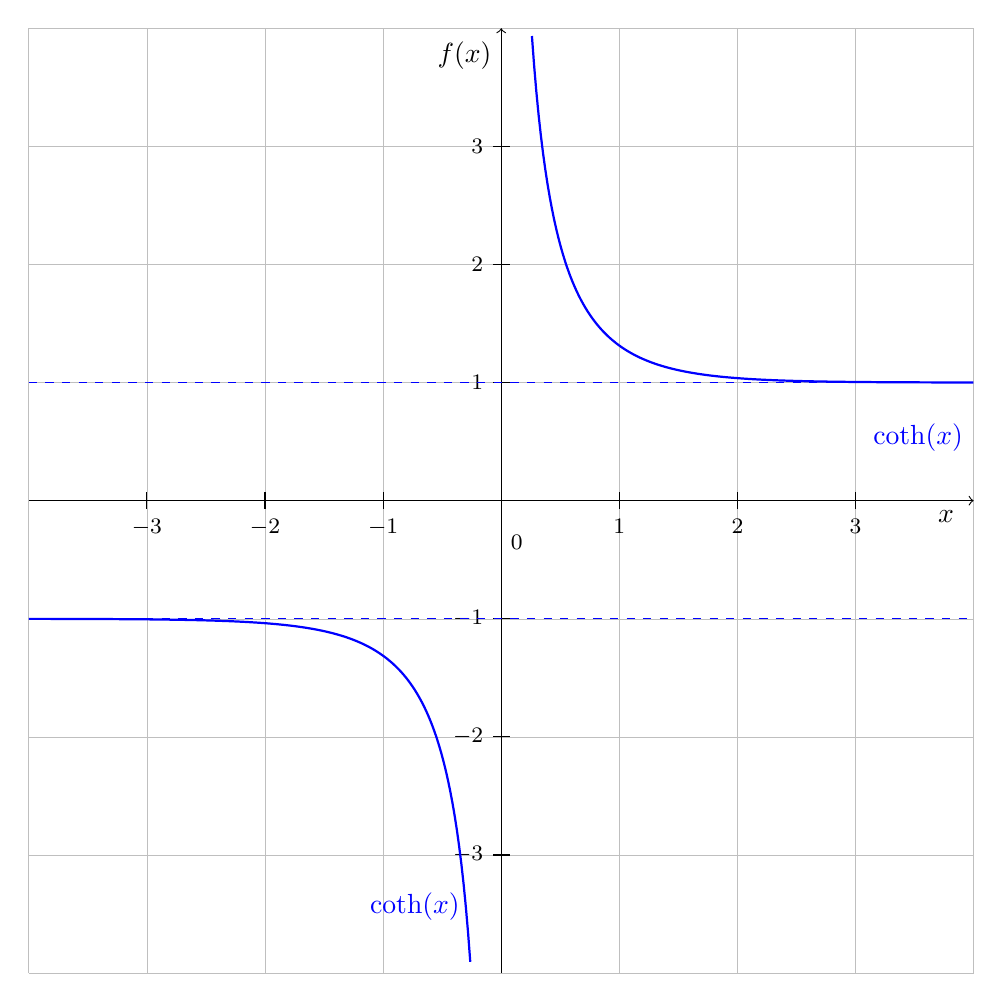
\begin{tikzpicture}[xscale=1.5, yscale=1.5]
	
	% Gitternetzlinien
	\draw[xstep=1cm, ystep=1cm, very thin, color=lightgray] (-4,4) grid (4,-4);
	% x-Achse
	\draw[->] (-4,0) -- (4,0) node[below,xshift=-1em] {$x$}; 
	%Zahlen auf x-Achse
	\foreach \x in {-3,...,-1}
	\draw[shift={(\x,0)},color=black] (0pt,2pt) -- (0pt,-2pt) node[below] {\footnotesize $\x$};
	\foreach \x in {1,...,3}
	\draw[shift={(\x,0)},color=black] (0pt,2pt) -- (0pt,-2pt) node[below] {\footnotesize $\x$};
	% y-Achse 
	\draw[->] (0,-4) -- (0,4) node[left,yshift=-1em] {$f(x)$};%node[above left]
	%Zahlen auf y-Achse
	\foreach \y in {-3,...,-1}
	\draw[shift={(0,\y)},color=black] (2pt,0pt) -- (-2pt,0pt) node[left] {\footnotesize $\y$};
	\foreach \y in {1,...,3}
	\draw[shift={(0,\y)},color=black] (2pt,0pt) -- (-2pt,0pt) node[left] {\footnotesize $\y$};
	%Ursprung
	\draw[color=black] (0pt,-10pt) node[right] {\footnotesize $0$};
	\draw[thick,color=blue] plot[samples=200, domain=-4.0:-.26] 
	(\x,{cosh(\x )/sinh(\x)}) node[yshift=2em, xshift=-2em] {$\coth(x)$};
	\draw[thick,color=blue] plot[samples=200, domain=.26:4] 
	(\x,{cosh(\x )/sinh(\x)}) node[yshift=-2em, xshift=-2em] {$\coth(x)$};
	
	\draw[color=blue,dashed] (-4,1)--(4,1);
	\draw[color=blue,dashed] (-4,-1)--(4,-1);
	
	
	%		\draw[thick,color=blue] plot[samples=200, domain=-2:2] 
	%	(\x,{sinh(\x )}) node[yshift=1, xshift=2.5em] {$\arcsin(x)$};
	%	\draw[color=black] (2pt,3.14) -- (-2pt,3.14) node[left] {\footnotesize $\pi$};
	\end{tikzpicture}\\
	\begin{align*}
	\coth:\mathbb{R}\backslash\{0\}\longmapsto \mathbb{R}\backslash \{-1,1\}
	\end{align*}
	
\end{center}
\begin{align*}
\mathrm{arcoth}:\;]-\infty,-1[\; \cup\;]1,\infty[\;\longmapsto \mathbb{R}\setminus \{0\}\\
\end{align*}
\begin{center}
	\begin{tikzpicture}[xscale=2, yscale=2]
	
	% Gitternetzlinien
	\draw[xstep=1cm, ystep=1cm, very thin, color=lightgray] (-4,2) grid (4,-2);
	% x-Achse
	\draw[->] (-4,0) -- (4,0) node[below,xshift=-1em] {$x$}; 
	%Zahlen auf x-Achse
	\foreach \x in {-3,...,-1}
	\draw[shift={(\x,0)},color=black] (0pt,2pt) -- (0pt,-2pt) node[below] {\footnotesize $\x$};
	\foreach \x in {1,...,3}
	\draw[shift={(\x,0)},color=black] (0pt,2pt) -- (0pt,-2pt) node[below] {\footnotesize $\x$};
	% y-Achse 
	\draw[->] (0,-2) -- (0,2) node[left,yshift=-1em] {$f(x)$};%node[above left]
	%Zahlen auf y-Achse
	\foreach \y in {-1,...,-1}
	\draw[shift={(0,\y)},color=black] (2pt,0pt) -- (-2pt,0pt) node[left] {\footnotesize $\y$};
	\foreach \y in {1,...,1}
	\draw[shift={(0,\y)},color=black] (2pt,0pt) -- (-2pt,0pt) node[left] {\footnotesize $\y$};
	%Ursprung
	\draw[thick,color=blue] plot[samples=200, domain=1.0009:4] 
	(\x,{(0.5*ln(sqrt((1+\x)/(\x-1)))});
	\draw[thick,color=blue] plot[samples=200, domain=-4:-1.00009] 
	(\x,{(0.5*ln(sqrt((1+\x)/(\x-1)))}) node[yshift=2, xshift=-3em] {$\mathrm{arcoth}(x)$};
	
	%\draw[thick,color=blue] plot[samples=200, domain=0:2.05] 
	%	(\x,{cosh(\x )}) node[yshift=-2em, xshift=2em] {$\cosh(x)$};
	%	\draw[color=blue,thick] (0pt,0pt) node {$[$};
	%\draw[color=blue,thick] (3.14,0pt) node { $]$};
	%	\draw[color=blue,thick] (0,0pt)--(4,0);
	
	\end{tikzpicture}\\	
\end{center}
Die Ableitung von Areakotangens Hyperbolicus:\\
\begin{align*}
\mathrm{arcoth}'(x)=-\frac{1}{1-x^2}
\end{align*}
\subsubsection{Aufgabe 1 zu Area-Funktionen}
\href{https://youtu.be/fkV0enqPc9E}{Video 17}\\
Zeige für $ x\in \mathbb{R} $ gilt $\mathrm{arsinh}=\ln(x+\sqrt{x^2+1})$.\\
Beweis:\\
Es gilt:\\
\begin{align*}
f(x)=\mathrm{arsinh}(x)-\ln(x+\sqrt{x^2+1})=0
\end{align*}
Wenn dies gelten soll, muß die Ableitung von $ f(x) $ konstant sein , denn $ f(x) $ muss ja Null sein wenn $\mathrm{arsinh}=\ln(x+\sqrt{x^2+1})  $ gelten soll.\\
\begin{align*}
f'(x)&=\mathrm{arsinh}'(x)-\big (\ln(x+\sqrt{x^2+1})\big )'\\
&=\frac{1}{\sqrt{x^2+1}}-\frac{1}{x+\sqrt{x^2+1}}\big(x+\sqrt{x^2+1}\big)'\\
&=\frac{1}{\sqrt{x^2+1}}-\frac{1}{x+\sqrt{x^2+1}}\bigg(1+\frac{1}{2\sqrt{x^2+1}}\cdot 2x\bigg)\\
&=\frac{1}{\sqrt{x^2+1}}-\frac{1}{x+\sqrt{x^2+1}}\bigg(1+\frac{x}{\sqrt{x^2+1}}\bigg)\\
&=\frac{1}{\sqrt{x^2+1}}-\frac{1}{x+\sqrt{x^2+1}}\bigg(\frac{\sqrt{x^2+1}+x}{\sqrt{x^2+1}}\bigg)\\
&=\frac{1}{\sqrt{x^2+1}}-\frac{x+\sqrt{x^2+1}}{(x+\sqrt{x^2+1})(\sqrt{x^2+1})}\\
&=\frac{x+\sqrt{x^2+1}-(x+\sqrt{x^2+1})}{(\sqrt{x^2+1})(x+\sqrt{x^2+1})}=0\\
\end{align*}
D.h.: $ f'(x)=0 $ für $ x\in \mathbb{R} \overset{\tiny Konstanzkriterium}{\longmapsto} f(x)=k\in\mathbb{R} $ für alle $ x\in \mathbb{R} $\\
Es gilt für $ f(0) $:\\
\begin{align*}
f(0)=\mathrm{arsinh}(0)-\ln(0+\sqrt{0^2+1})=0
\end{align*}
\begin{align*}
&0\overset{\mathrm{sinh}}{\longmapsto} 0\\
&0\overset{\mathrm{arsinh}}{\longmapsto} 0\\
\end{align*}
\subsubsection{Aufgabe 2 zu Area-Funktionen}
\href{https://youtu.be/y-3Ng9HCIEo}{Video 18}\\
Zeige für $ x\geq 1 $ gilt $\mathrm{arcosh}=\ln(x+\sqrt{x^2-1})$.\\
Beweis:\\
Es gilt:\\
\begin{align*}
g(x)=\mathrm{arcosh}(x)-\ln(x+\sqrt{x^2-1})=0
\end{align*}
Für $ x>1 $ gilt:
\begin{align*}
g'(x)&=\mathrm{arcosh}'(x)-\big(\ln(x+\sqrt{x^2-1})\big)'\\
&=\frac{1}{\sqrt{x^2-1}}-\frac{1}{x+\sqrt{x^2-1}}\big(x+\sqrt{x^2-1}\big)'\\
&=\frac{1}{\sqrt{x^2-1}}-\frac{1}{x+\sqrt{x^2-1}}\bigg(1+\frac{x}{\sqrt{x^2-1}}\bigg)\\
&=\frac{1}{\sqrt{x^2-1}}-\frac{\sqrt{x^2-1}+x}{(x+\sqrt{x^2-1})(\sqrt{x^2-1})}\\
&=\frac{x+\sqrt{x^2-1}-(\sqrt{x^2-1}+x)}{(x+\sqrt{x^2-1})(\sqrt{x^2-1})}=0
\end{align*}
D.h.: $ g'(x)=0 $ für $ x>1 \overset{\tiny Konstanzkriterium}{\longmapsto} g(x)=k\in\mathbb{R} $ für alle $ x \geq 1 $\\
Es gilt für $ g(1) $:\\
\begin{align*}
k=g(1)=\mathrm{arcosh}(1)-\ln(x+\sqrt{1^2-1})=0
\end{align*}
\begin{align*}
&0\overset{\mathrm{cosh}}{\longmapsto} 1\\
&1\overset{\mathrm{arcosh}}{\longmapsto} 0\\
\end{align*}
\subsection{Die Exponentialfunktion}
\href{https://youtu.be/au-TAWRpb3Y}{Video 19}\\
Es gibt genau eine diffbar. Funktion $ \exp:\mathbb{R}\longmapsto \mathbb{R}_{>0} $ mit \\
\begin{align*}
\exp'(x)=\exp(x)\;\;\text{und }\;\;\exp(0)=1 .
\end{align*}
Diese Funktion heißt Eponentialfunktion, wobei gilt:\\
\begin{align*}
&\mathrm{e}^x:=\exp(x)\\
&\mathrm{e}=\exp(1)=2.7182\ldots\in\mathbb{R}\backslash \mathbb{Q}\\
\end{align*}
Bemerkung:\\
$\mathbb{R}\backslash \mathbb{Q}  $ sind die irrationalen Zahlen . Ist die Menge aller Elemente von $ \mathbb{R} $, die nicht in  $\mathbb{Q}$ liegen.\\
\\
Wegen $ \big(\mathrm{e}^x\big)'=\mathrm{e}^x>0 \overset{Monotoniekr.}{\Longrightarrow} \mathrm{e}^x$ ist streng monoton wachsend\\
\begin{center}
	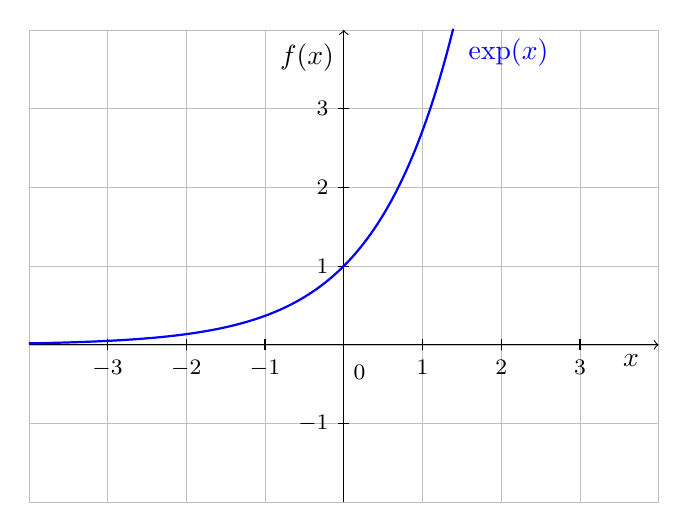
\begin{tikzpicture}[xscale=1, yscale=1]
	
	% Gitternetzlinien
	\draw[xstep=1cm, ystep=1cm, very thin, color=lightgray] (-4,4) grid (4,-2);
	% x-Achse
	\draw[->] (-4,0) -- (4,0) node[below,xshift=-1em] {$x$}; 
	%Zahlen auf x-Achse
	\foreach \x in {-3,...,-1}
	\draw[shift={(\x,0)},color=black] (0pt,2pt) -- (0pt,-2pt) node[below] {\footnotesize $\x$};
	\foreach \x in {1,...,3}
	\draw[shift={(\x,0)},color=black] (0pt,2pt) -- (0pt,-2pt) node[below] {\footnotesize $\x$};
	% y-Achse 
	\draw[->] (0,-2) -- (0,4) node[left,yshift=-1em] {$f(x)$};%node[above left]
	%Zahlen auf y-Achse
	\foreach \y in {-1,...,-1}
	\draw[shift={(0,\y)},color=black] (2pt,0pt) -- (-2pt,0pt) node[left] {\footnotesize $\y$};
	\foreach \y in {1,...,3}
	\draw[shift={(0,\y)},color=black] (2pt,0pt) -- (-2pt,0pt) node[left] {\footnotesize $\y$};
	%Ursprung
	\draw[color=black] (0pt,-10pt) node[right] {\footnotesize $0$};
	
	
	\draw[thick,color=blue] plot[samples=200, domain=-4:1.39] 
	(\x,{e^\x}) node[below, xshift=2em]{$\exp(x)$};
	
	
	
	\end{tikzpicture}\\
\end{center}
Es gilt das Taylorpolynom:\\
\begin{align*}
\exp(x)=\mathrm{e}^x=\sum\limits_{k=0}^{n}\frac{x^k}{k!}+\mathrm{R}_n(x)
\end{align*}
\underline {Grenzwertbetrachtungen:}
\begin{quote}
	\begin{align*}
	&\lim\limits_ {n\to\infty}\frac{\mathrm{e}^x}{x^n}=\infty\;\;\text{für }\;\;n\in\mathbb{N}\\
	&\lim\limits_ {n\to-\infty}|x^n|\cdot\mathrm{e}^x=0\;\;\text{für }\;\;n\in\mathbb{N}\\
	\end{align*}
	Die Exponentialfunktion wächst schneller gegen Unendlich als jede Potenz von $ x $.\\
	Ebenso geht sie bei Minusunendlich schneller gegen Null als der Betrag von der Potenz von $ x $ wächst.\\
\end{quote}
\underline{Eigenschaften:}\\
Für $ x,y\in\mathbb{R} $ gilt:\\
\begin{align*}
&\mathrm{e}^x\cdot \mathrm{e}^y=\mathrm{e}^{x+y}\\
&\mathrm{e}^{-x}=\frac{1}{\mathrm{e}^x}
\end{align*}
\underline{Für die allgemeine Exponentialfunktion gilt:}\\
Für $ a>0  $ definiert man:\\
\begin{align*}
a^x:=\mathrm{e}^{\ln(a)\cdot x}
\end{align*}
$ a $ nennt man Basis\\
$ x $ nennt man Exponent\\
Wegen $ (-1)^{\genfrac{}{}{}{2}{1 }{2 }} =\sqrt{-1}$ muß $ a>0 $ sein. Negative Wurzel! \\
Für $ 0<a<1 $ ist $ a^x $ streng monoton fallend.\\
Für $ a>1 $ ist $ a^x $ streng monoton wachsend.\\
\begin{center}
	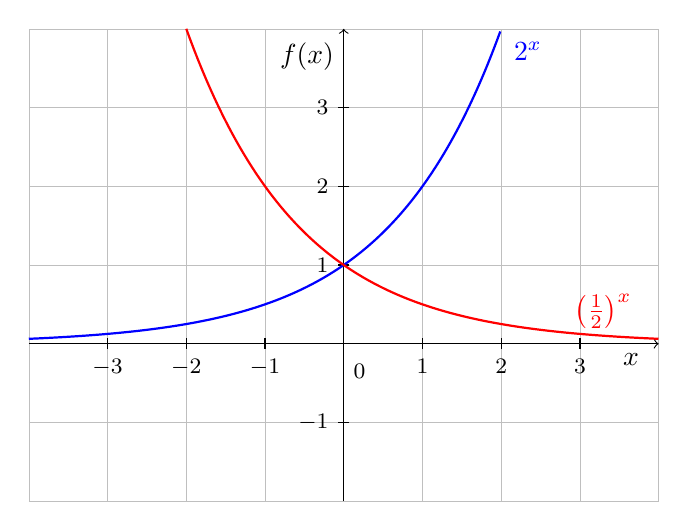
\begin{tikzpicture}[xscale=1, yscale=1]
	
	% Gitternetzlinien
	\draw[xstep=1cm, ystep=1cm, very thin, color=lightgray] (-4,4) grid (4,-2);
	% x-Achse
	\draw[->] (-4,0) -- (4,0) node[below,xshift=-1em] {$x$}; 
	%Zahlen auf x-Achse
	\foreach \x in {-3,...,-1}
	\draw[shift={(\x,0)},color=black] (0pt,2pt) -- (0pt,-2pt) node[below] {\footnotesize $\x$};
	\foreach \x in {1,...,3}
	\draw[shift={(\x,0)},color=black] (0pt,2pt) -- (0pt,-2pt) node[below] {\footnotesize $\x$};
	% y-Achse 
	\draw[->] (0,-2) -- (0,4) node[left,yshift=-1em] {$f(x)$};%node[above left]
	%Zahlen auf y-Achse
	\foreach \y in {-1,...,-1}
	\draw[shift={(0,\y)},color=black] (2pt,0pt) -- (-2pt,0pt) node[left] {\footnotesize $\y$};
	\foreach \y in {1,...,3}
	\draw[shift={(0,\y)},color=black] (2pt,0pt) -- (-2pt,0pt) node[left] {\footnotesize $\y$};
	%Ursprung
	\draw[color=black] (0pt,-10pt) node[right] {\footnotesize $0$};
	
	
	\draw[thick,color=blue] plot[samples=200, domain=-4:1.99] 
	(\x,{2^\x}) node[below, xshift=1em]{$2^x$};
	\draw[thick,color=red] plot[samples=200, domain=-2:4] 
	(\x,{0.5^\x}) node[below, yshift=2em,xshift=-2em]{$\big(\frac{1}{2}\big)^x$};
	
	
	\end{tikzpicture}\\
\end{center}
Die Achsen-Symmetrie: $ f(x)=f(-x) $ gilt hier wegen:\\
\begin{align*}
\bigg(\frac{1}{2}\bigg)^x=2^{-x}
\end{align*}
\underline{Ableitung}\\
\begin{align*}
(a^x)'=\bigg(\mathrm{e}^{\ln(a)x}\bigg)'=\mathrm{e}^{\ln(a)x}\cdot(\ln(a)x)'=a^x\ln(a)\\
\end{align*}
Bemerkung:\
$ \ln(a) $ ist für $ a<1 $ negativ daraus folgt $ a^x $ ist monoton fallend.\\
\underline{Rechenregeln:}
\begin{align*}
&a^x=\mathrm{e}^{\ln(a)x}\\
&\big(a^b\big)^c=a^{b\cdot c}\\
&\sqrt{x^7}=\big(x^7\big)^{\frac{1}{2}}=x^{\frac{7}{2}}=(\sqrt{x})^7
\end{align*}
\subsubsection{Der Logarithmus}
\href{https://youtu.be/gCVOSyUEYIk}{Video 20}\\
Der Logarithmus ist das Gegenstück zur Exponentialfunktion.\\
Der natürliche Logarithmus ist die Umkehrfunktion von der Eponentialfunktion.
\begin{align*}
\exp:\mathbb{R}\longmapsto \;]0,\infty[ 
\end{align*}\\
D.h.:
\begin{align*}
\ln:\;]0,\infty[ \;\longmapsto \mathbb{R} \;\;\text{mit }\;\;x\longmapsto \exp^{-1}(x)=\ln(x)
\end{align*}
\begin{center}
	
	
	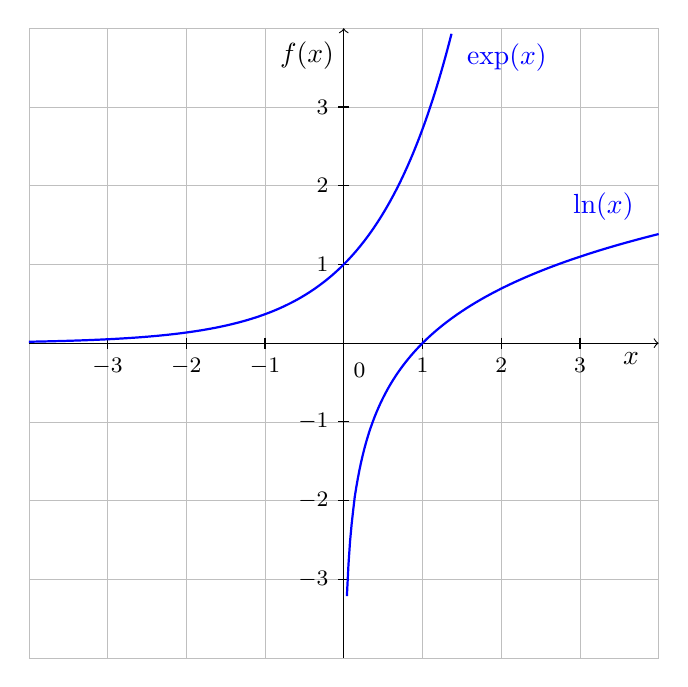
\begin{tikzpicture}[xscale=1, yscale=1]
	
	% Gitternetzlinien
	\draw[xstep=1cm, ystep=1cm, very thin, color=lightgray] (-4,4) grid (4,-4);
	% x-Achse
	\draw[->] (-4,0) -- (4,0) node[below,xshift=-1em] {$x$}; 
	%Zahlen auf x-Achse
	\foreach \x in {-3,...,-1}
	\draw[shift={(\x,0)},color=black] (0pt,2pt) -- (0pt,-2pt) node[below] {\footnotesize $\x$};
	\foreach \x in {1,...,3}
	\draw[shift={(\x,0)},color=black] (0pt,2pt) -- (0pt,-2pt) node[below] {\footnotesize $\x$};
	% y-Achse 
	\draw[->] (0,-4) -- (0,4) node[left,yshift=-1em] {$f(x)$};%node[above left]
	%Zahlen auf y-Achse
	\foreach \y in {-1,...,-3}
	\draw[shift={(0,\y)},color=black] (2pt,0pt) -- (-2pt,0pt) node[left] {\footnotesize $\y$};
	\foreach \y in {1,...,3}
	\draw[shift={(0,\y)},color=black] (2pt,0pt) -- (-2pt,0pt) node[left] {\footnotesize $\y$};
	%Ursprung
	\draw[color=black] (0pt,-10pt) node[right] {\footnotesize $0$};
	
	\draw[thick,color=blue] plot[samples=200, domain=-4:1.37] 
	(\x,{e^\x}) node[below, xshift=2em] {$\exp(x)$};
	
	\draw[thick,color=blue] plot[samples=200, domain=0.04:4] 
	(\x,{ln(\x)}) node[yshift=1em,xshift=-2em]{$\ln(x)$};
	
	
	
	\end{tikzpicture}\\
\end{center}
\pagebreak
Eigenschaften:\\
\begin{quote}
	Sei $ x,y\in\;]0,\infty[ $\\
	\begin{align*}
	&\text{(i) }\;\;\ln(x\cdot y)=\ln(x)+\ln(y)\\
	\\
	&\text{(ii) }\;\ln(x^\alpha) =\alpha\cdot \ln(x)\;\;\text{für }\;\;\alpha\in\mathbb{R})\\
	\\
	&\text{(iii) }\lim\limits_ {x\to\infty}\ln(x)=\infty  \\
	&\;\;\;\;\;\;\;\;\lim\limits_ {\substack{x\mapsto 0\\x>0}}\ln(x)=-\infty\\
	\end{align*}
\end{quote}
Für den Logarithmus zur Basis $ a $ mit $ a>0 $ gilt:\\
\begin{align*}
\log_a(x)=\frac{\ln(x)}{\ln(a)}=y
\end{align*}
Die Umkehrfunktion von der allgemeinen Exponentialfunktion: $ a^x $ ist der Logarithmus: $\log_a(x) $.\\
Beweis:\\
Es gilt die Eigenschaft der Umkehrabbildung:\\
\begin{align*}
f(x)\circ f^{-1}(x)=x=f^{-1}(x)\circ f(x)\\
\end{align*}
Dann gilt für: $ f(x)=a^x=\mathrm{e}^{\ln(a)x}$  und $f^{-1}(x)=\log_a(x) $:\\
\begin{align*}
f(x)\circ f^{-1}(x)&=\mathrm{e}^{\ln(a)(\log_a(x)}=\mathrm{e}^{\ln(a)\frac{\ln(x)}{\ln(a)}}=\mathrm{e}^{\ln(x)}=x_{_{\Square}}\\
\end{align*}
Eigenschaften:\\
\begin{quote}
	Sei $ a,b,c>0\in \mathbb{R}  $ und $ \alpha\in\;]0,\infty[ $\\
	\begin{align*}
	&\text{(i) }\;\;\log_a(b)\cdot \log_b(c)=\frac{\ln(b)}{\ln(a)}\cdot\frac{\ln(c)}{\ln(b)}=\frac{\ln(c)}{\ln(a)}=\log_a(c)\\
	\\
	&\text{(ii) }\lim\limits_ {x\to\infty}\frac{\ln(x)}{x^\alpha}=0 \;\;\text{für }\;\;\alpha=\in\;]0,\infty[\\
	&\;\;\;\;\;\;\lim\limits_ {x\to\infty}\frac{\ln(x)}{\sqrt{x}}=0\;\;\text{für }\;\;\alpha=\frac{1}{2}\\
	\end{align*}
\end{quote}
\underline{Kategorien des Wachstums von Funktionen:}\\
\begin{quote}
	1. Exponentielle $ \mathrm{e}^x,\; a^x $\\
	2. Polynominelle $ x^n,\;\; n\in\mathbb{N} $ (für $ n=1  $ : Funktion ist linear.)\\
	3. Wurzel $ \sqrt[k]{x},\;\; k\in\mathbb{N}\backslash \{0\} $
\end{quote}
\subsubsection{Aufgabe zum Thema Exponentialfunktion und Logarithmus Teil 1+2}
\href{https://youtu.be/g6oiy5HrFNo}{Video 21}\\
Bestimme den maximalen Definitionsbereich, die Ableitung und das Bild von:\\
\begin{align*}
f(x)=x^{\big(\sqrt{x}^x\big)}\\
\end{align*}
\underline{Maximaler Definitionsbereich:}\\
\begin{align*}
\mathbb{D}_f=[0,\infty[
\end{align*}
\underline{Das Bild von f:}\\
\begin{quote}
	(i)\;\;$ f(0)=0^{\big(\sqrt{0}^0\big)}=0^{(0^0)}=0^1=0 $\\
	\\
	(ii)\;$ f(x)\geq 0 $ für alle $ x\in \mathbb{D}_f $\\
	\\
	(iii)$ \lim\limits_ {x\to\infty}x^{\big(\sqrt{x}^x\big)}=\;\;? $\\
	\begin{quote}
		$ f(x)=x^{\big(\sqrt{x}^x\big)}=\mathrm{e}^{\ln(x)\cdot \sqrt{x}^x}=\mathrm{e}^{\ln(x)\cdot x^{\genfrac{}{}{}{2}{x }{2 }}} $\\
		$ \lim\limits_ {x\to\infty}f(x)=\lim\limits_ {x\to\infty}\mathrm{e}^{\ln(x)\cdot x^{\frac{x}{2}}} =\infty $	
	\end{quote}
	Fazit: Wegen (i), (ii) und (iii) folgt:\\
	\begin{align*}
	\mathrm{Bild}(f)=[0,\infty[
	\end{align*}
\end{quote}
\newpage
\noindent
\href{https://youtu.be/qDxy5Th1pfc}{Video 22}\\
\underline{Die Ableitung von $ f(x) $:}\\
\begin{align*}
f'(x)&=\bigg(x^{(\sqrt{x}^x)}\bigg)'=\bigg(\mathrm{e}^{\ln(x)\cdot x^{\frac{x}{2}}}\bigg)'\\
&=\mathrm{e}^{\ln(x)\cdot x^{\frac{x}{2}}}\cdot\big(\ln(x)\cdot x^{\frac{x}{2}}\big)'\\
&=\mathrm{e}^{\ln(x)\cdot x^{\frac{x}{2}}}\cdot \big[\ln'(x)\cdot x^{\frac{x}{2}}+\big(x^{\frac{x}{2}}\big)'\cdot \ln(x)\big]\\
&=\mathrm{e}^{\ln(x)\cdot x^{\frac{x}{2}}}\cdot\bigg[\frac{1}{x}\cdot x^{\frac{x}{2}}+\big(\mathrm{e}^{\ln(x)\cdot \frac{x}{2}}\big)'\ln(x)\bigg]\\
&=\mathrm{e}^{\ln(x)\cdot x^{\frac{x}{2}}}\cdot\bigg[\frac{1}{x}\cdot x^{\frac{x}{2}}+\big[\mathrm{e}^{\ln(x)\cdot \frac{x}{2}}(\genfrac{}{}{}{2}{1 }{x }\cdot \genfrac{}{}{}{2}{x }{2 }+\ln(x)\cdot \genfrac{}{}{}{2}{1}{2 })\big]\ln(x)\bigg]\\
&=\mathrm{e}^{\ln(x)\cdot x^{\frac{x}{2}}}\cdot \bigg[\frac{1}{x}\cdot x^{\frac{x}{2}}+\big[ x^{\frac{x}{2}}(\genfrac{}{}{}{2}{1 }{2 }+ \genfrac{}{}{}{2}{\ln(x)}{2 })\big]\ln(x)\bigg]\\
&=\mathrm{e}^{\ln(x)\cdot x^{\frac{x}{2}}}\cdot\bigg[\frac{1}{x}\cdot x^{\frac{x}{2}}+\big[\genfrac{}{}{}{2}{1 }{2} x^{\frac{x}{2}}(1+ \ln(x))\big]\ln(x)\bigg]\\
&=\mathrm{e}^{\ln(x)\cdot x^{\frac{x}{2}}}\cdot x^{\frac{x}{2}}\bigg[\genfrac{}{}{}{2}{1 }{x }+\big[\genfrac{}{}{}{2}{\ln(x) }{2 }(1+\ln(x)\big ]\bigg ]\\
&=x^{(\sqrt{x}^x)}\cdot x^{\frac{x}{2}}\bigg[\genfrac{}{}{}{2}{1 }{x }+\big[\genfrac{}{}{}{2}{\ln(x) }{2 }(1+\ln(x)\big ]\bigg ]\\
&=x^{\big(\sqrt{x}^x+x^{\frac{x}{2}}\big)}\bigg[\genfrac{}{}{}{2}{1 }{x }+\big[\genfrac{}{}{}{2}{\ln(x) }{2 }(1+\ln(x)\big ]\bigg ]\\
\end{align*}
\subsubsection{ Lösen von Gleichungen mittels der Exponentialfunktion und dem Logarithmus}
\href{https://youtu.be/w04eRCcWpHU}{Video 23}\\
Bestimme alle Lösungen von:\\
\begin{align*}
4^{4x}=2^{6x}\cdot 4^x\cdot 256^{x-1}
\end{align*}
Gleiche Basen erzeugen:\\
\begin{align*}
\Leftrightarrow \big(2^2\big)^{4x}=2^{6x}\cdot \big(2^2\big)^{x}\cdot\big(2^8\big)^{x-1}
\end{align*}
Anwendung von: $ \big(a^b\big)^c=a^{a\cdot c} $\\
\begin{align*}
\Leftrightarrow  2^{2\cdot 4x}=2^{6x}\cdot 2^{2x}\cdot 2^{8(x-1)}
\end{align*}
Anwendung von: $ a^b\cdot a^c=a^{a+b} $\\
\begin{align*}
\Leftrightarrow 2^{8x}=2^{6x+2x+8(x-1)}=2^{16x-8}\\
\end{align*}
Mit $ 2^{8x} $ teilen.\\
\begin{align*}
\Leftrightarrow 1&=2^{16x-8}\cdot 2^{-8x}\\
&=2^{8x-8}
\end{align*}
Mit $ 1=2^0 $ ergibt:\\
\begin{align*}
\Leftrightarrow2^0=2^{8x-8}\\
\end{align*}
Mit $ \log_2(...) $ ergibt:\\
\begin{align*}
\Leftrightarrow \log_2(2^0)&=\log_2\big(2^{(8x-8)}\big)\\
\end{align*}
Anwendung von: $ \log(a^b)=b\log(a) $
\begin{align*}
\log_2(2^0)&=(8x-8)\log_2(2)\\
0&=8x-8\\
\Leftrightarrow 8x&=8\\
\Leftrightarrow x&=1
\end{align*}
Fazit: $ x=1 $ ist die einzigste Lösung.\\